\documentclass[english]{beamer}
\usepackage{mathptmx}
\usepackage[T1]{fontenc}
\usepackage[latin9]{inputenc}
\usepackage{url}
\usepackage{amsmath}
\usepackage{amssymb}
\usepackage{graphicx}
\usepackage{mathtools}
\usepackage{dsfont}
\usepackage{hyperref}

\makeatletter
\newcommand\makebeamertitle{\frame{\maketitle}}%
\AtBeginDocument{%
  \let\origtableofcontents=\tableofcontents
  \def\tableofcontents{\@ifnextchar[{\origtableofcontents}{\gobbletableofcontents}}
  \def\gobbletableofcontents#1{\origtableofcontents}
}
\setbeamertemplate{navigation symbols}{%
    \usebeamerfont{footline}%
    \usebeamercolor[fg]{footline}%
    \hspace{1em}
}
\setbeamercolor{footline}{fg=black}
\setbeamerfont{footline}{series=\bfseries}
\setbeamercolor{frametitle}{fg=blue}
\setlength{\leftmargini}{5pt}

\usepackage{lmodern}

\makeatother

\usepackage{babel}

 
\begin{document}

\title{\textcolor{blue}{Text Analysis for Economics and Finance}}
\vspace{8pt} 
\author{Ruben Durante\\
\small{ICREA-UPF, BGSE, IPEG, CEPR}}
\date{\small{DIW, October 2020}}

\frame{\titlepage}
\setbeamercovered{dynamic}

\begin{frame}{Introduction}

\begin{itemize}
\setlength{\itemsep}{0.9em}
\item Applied work in social sciences, and economics in particular, relies heavily on quantitative
data (e.g., prices, quantities, votes, etc.)

\item Large amounts of text generated in socioeconomic environments (e.g., company reports, news articles, committee deliberations, political speeches, court decisions)

\item These data can be used qualitatively, but increasing interest in treating text quantitatively, also due to advances in computing power and software capabilities

\item Great possibilities but also great challenges

\pause

\item How to apply standard statistical methods to \textcolor{blue}{unstructured} text?

\end{itemize}
\end{frame}


\begin{frame}{Aim of the course}

\begin{itemize}
    \item Introduction to the use of text data for research in economics and finance
\vspace{10pt}
    \item Goals:
\vspace{8pt}
\begin{itemize}
\setlength{\itemsep}{0.9em}
\setlength{\itemindent}{-0.8em}

    \item Think about \textcolor{blue}{research questions} that text data can help answering
    \item \textcolor{blue}{Prepare text corpora}, transform them into matrices of text features
    \item Apply adequate statistical methods for descriptive and causal analysis
    \item In depth discussion of \textcolor{blue}{applications} from different fields
    
\end{itemize}

\end{itemize}
\end{frame}

\begin{frame}{Material}

\begin{itemize}
\setlength{\itemsep}{0.7em}
    \item  Slides; articles, surveys and book chapters mentioned in slides
    \vspace{4pt}
\begin{itemize}
\setlength{\itemsep}{0.7em}
\setlength{\itemindent}{-0.8em}
    \item  Gentzkow, M., et al., 2017, Text as Data, NBER WP \#23276.
    \item  Manning, C. D., et al., An Introduction to Information Retrieval,\\
\hspace{-8pt}Cambridge University Press.
    \item Grimmer, J. and Stewart, B., 2013, Text as Data: The Promise and\\
\hspace{-8pt}Pitfalls of Automatic Content Analysis Methods for Political Texts,\\
\hspace{-8pt}Political Analysis.
\item Bengfort, B. et al., Applied Text Analysis with Python, 2018,\\
\hspace{-8pt}O'Reilly Media
\end{itemize}
\item See syllabus for other recommended readings
\end{itemize}
\end{frame}

\begin{frame}{Course organization}
\begin{itemize}
\setlength{\itemsep}{1em}
%\setlength{\itemindent}{-0.8em}
    \item  \textcolor{blue}{Instructors}: 
    \vspace{4pt}
    \begin{itemize}
    \setlength{\itemsep}{0.6em}
    \item Ruben Durante (ICREA-UPF, BGSE): \textcolor{blue}{ruben.durante@upf.edu}
    \end{itemize}
    \item \textcolor{blue}{Activities}: 12 hours of lecture, 3 hours of practical sessions.
    \item  \textcolor{blue}{Evaluation}: Class participation, final project
   \item  \textcolor{blue}{Final project}: ideally a question that is relevant to your thesis or research agenda and could develop into a paper
\end{itemize}
\end{frame}

\begin{frame}{New Data, New Possibilities}
\begin{figure}[h]
\begin{centering}
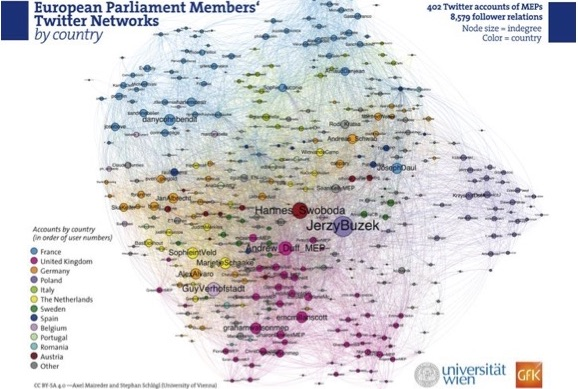
\includegraphics[height=2.7in]{Images/fig2}
\end{centering}
\end{figure}
\end{frame}

\begin{frame}{New Data, New Challenges}
\begin{itemize}
\item   What do we do with millions (or billions) of rows like this?
\end{itemize}
\vspace{-15pt}
\begin{center}
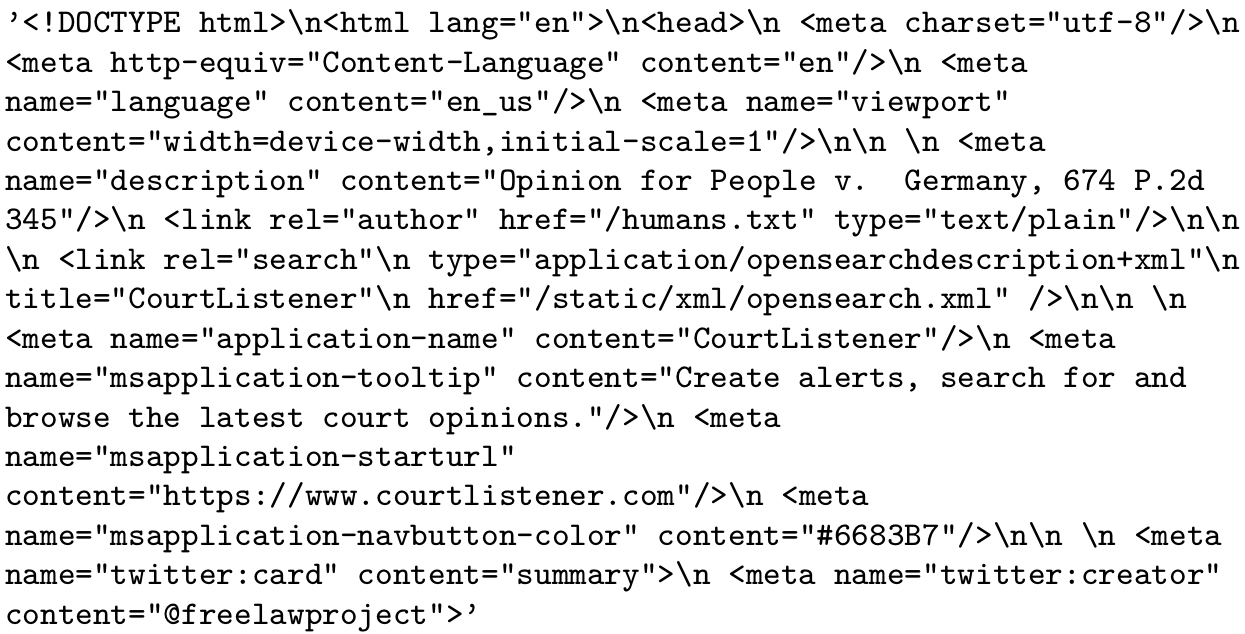
\includegraphics[height=2.3in]{Images/fig3}
\end{center}
\end{frame}

\begin{frame}{What is special about text data?}
\begin{itemize}
\setlength{\itemsep}{0.9em}
\item Text is inherently \textcolor{blue}{high dimensional}
\item A sample of 30-word Twitter messages using the 1,000 most common English words has as many dimensions as there are atoms in the universe!
\item Hence, the methods used to analyze text are related to those used to analyze high-dimensional data
\item Same as those used to analyze genetic data, big administrative health and tax data, credit data, online purchase data, etc.
\item Big effort to try to \textcolor{blue}{reduce dimensionality} to make the problem more manageable 

% (use high-dimensional statistical methods)
% 
%\item Use $\hat{V}$ in subsequent descriptive or causal analysis\\
%\vspace{2pt}
% (make predictions, infer causality, estimate structural parameters)
%\end{enumerate}
%
%\begin{itemize}
%\item \textcolor{blue}{Important}: use text to tackle an important question that would be hard to study otherwise
\end{itemize}

\end{frame}



\begin{frame}{The general problem}
\begin{enumerate}
\setlength{\itemsep}{1em}
\item Represent raw text ${D}$ as a numerical array $C$ \\
\vspace{2pt}
 (reduce dimensionality of the data)
 
\item Map $C$ to predicted values $\hat{V}$ of unknown outcome $V$\\
\vspace{2pt}
 (use high-dimensional statistical methods)
 
\item Use $\hat{V}$ in subsequent descriptive or causal analysis\\

\end{enumerate}

\vspace{5pt}

\begin{itemize}
\item \textcolor{blue}{Goals}: i) describe, ii) predict, iii) use as input for causal inference
\end{itemize}

\vspace{5pt}

\begin{itemize}
\item \textcolor{blue}{Important}: use text to tackle an important question that would be hard to study otherwise
\end{itemize}

\end{frame}

\begin{frame}{The general problem: example \#1}

\begin{enumerate}

\item We want to study how fear of Ebola affected voting behavior in the 2014 U.S. elections \textcolor{blue}{(Campante et al., 2020)}

\vspace{4pt}

\begin{itemize}

\setlength{\itemindent}{-0.9em}
\setlength{\itemsep}{1.5em}

\item We'd like to measure concern about Ebola by county and day. \\
\hspace{-9pt}But we can't!

\item We collect all the tweets mentioning Ebola with date and location

\item We construct measures of the frequency of Ebola tweets, look at\\
\hspace{-9pt}what emotions they express, and what words are mostly associated\\
\hspace{-9pt}with Ebola

\item Use these measures to study the causal impact of Ebola on voting\\
\hspace{-9pt}and the mechanism(s) through which it operates

\end{itemize}

\end{enumerate}

\end{frame}

\begin{frame}{The general problem: example \#2}

\begin{enumerate}
\item We want to understand how politicians' rhetoric affects voters' turnout

\vspace{7pt}

\begin{itemize}
\setlength{\itemindent}{-0.9em}
\setlength{\itemsep}{1.7em}
%\item We'd like to measure concern about Ebola by county and day ($\hat{V}$). \\
%\hspace{-9pt}But we can't!
 
\item We collect all the political speeches by different candidates

\item We construct measures of how they speak (e.g., length, complexity, \\
\hspace{-9pt}language), what they talk about (topic models), what emotions they \\
\hspace{-9pt}spur (sentiment analysis), etc.

\item Use these measure to illustrate differences (e.g., by party, gender, \\
\hspace{-9pt}age) and study how  political communication can mobilize voters

\end{itemize}

\end{enumerate}

\end{frame}

\begin{frame}{The general problem: more examples}

\begin{itemize}
\setlength{\itemsep}{1em}
\item Text of an email $\longrightarrow$ predict if it is spam or not
\item Text of a product review $\longrightarrow$ predict if it is positive or negative
\item Google searches $\longrightarrow$ predict incidence of local flu outbreaks
\item Google searches $\longrightarrow$ predict unemployment claims and retail sales
\item Text of news articles $\longrightarrow$ predict stock prices
\end{itemize}

\vspace{7pt}

\hspace{-15pt}In these examples the goal is just to \textcolor{blue}{predict $\hat{V}$}. In other cases $\hat{V}$ is\\
\hspace{-15pt}used as input for further analysis:

\vspace{7pt}

\begin{itemize}
\setlength{\itemsep}{1.3em}
\item E.g., use Google searches to estimate racial animus, and study how this influences voting for Obama (Stephens-Davidovitz, 2014)
\end{itemize}

\end{frame}

%2. Map C to predicted values Vˆ of
%unknown outcomes V; and
%3. Use Vˆ in subsequent descriptive or
%causal analysis.
%

\begin{frame}{NLP process: text $\rightarrow$ feature matrix $\rightarrow$ analysis}

\begin{figure}[h]
\begin{centering}
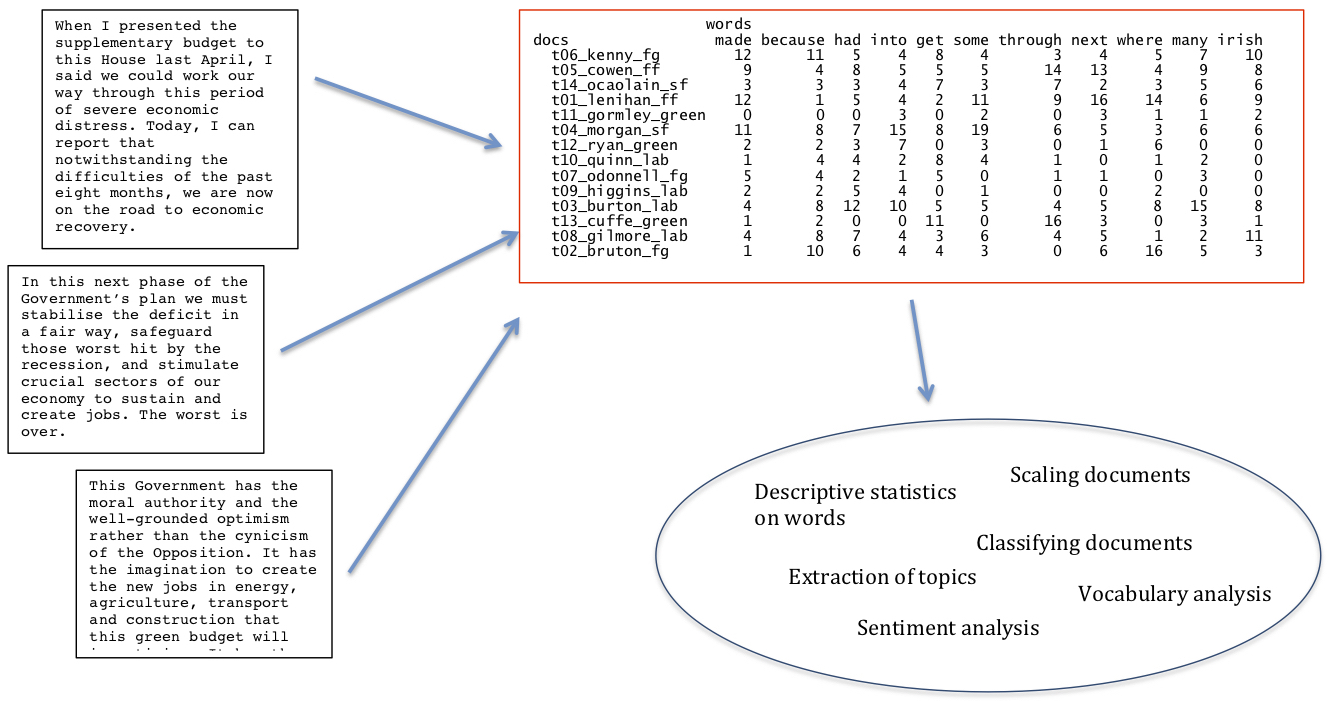
\includegraphics[height=2.4in]{Images/fig5}
\end{centering}
\end{figure}
\end{frame}

\begin{frame}{Useful concepts}

\begin{itemize}
\setlength{\itemsep}{1em}
\item The unit of analysis in a textual database is a \textcolor{blue}{document}.
\item The set of documents is the \textcolor{blue}{corpus}
\pause
\item Text data is \textcolor{blue}{unstructured}: the information we want is mixed with (lots) of other information we don't want
\item How to separate the two? All approaches will throw away some information, key to figure out how to retain the valuable one
\pause
\item Each document is associated with covariates which are usually called \textcolor{blue}{metadata}
\pause
\item E.g., in corpus on transcripts from the FOMC \small{(Hansen et al. 17)}: 
\vspace{4pt}
\begin{itemize}
\setlength{\itemsep}{0.3em}
\setlength{\itemindent}{-0.9em}
\item Document: statement by a speaker in a meeting
\item Metadata: date, speaker's bio info, economic variables at time, etc. 
\end{itemize}
\end{itemize}
\end{frame}

\begin{frame}{What counts as a document?}
\begin{itemize}
\setlength{\itemsep}{1em}
\item \textcolor{blue}{The unit of document analysis varies depending on the question}
\pause
\item If you are looking at how judges decide different types of cases, then \textcolor{blue}{a case} would be a document.
\pause
\item If you are looking at how judges differ within a court, then you might aggregate \textcolor{blue}{all of a judge's cases} as a document.
\pause
\item If you are looking at the impact of court cases on crime in a year, you might aggregate \textcolor{blue}{all the cases in a single year} as a single document. 
\pause
\item If you are looking at how different topics are discussed within single cases, then a document might be \textcolor{blue}{a section or a paragraph}.
\end{itemize}
\end{frame}

\begin{frame}{Possible data sources}
\begin{itemize}
\setlength{\itemsep}{0.8em}
\item Existing datasets:
\vspace{2pt}
\begin{itemize}
\setlength{\itemsep}{0.3em}
\item \textcolor{blue}{Parliamentary records}: UCD's EuroParl project, Hansard Archive of U.K. parliamentary debates, U.S. Congressional record
\item \textcolor{blue}{Media archives (newspaper articles, TV transcripts)}: e.g., LexisNexis, ProQuest, Factiva
\item \textcolor{blue}{Academic article}: JSTOR Data for Research, EconLit
\item Open-ended responses to survey questions
\end{itemize}
\pause
\item Collect your own data:
\vspace{2pt}
\begin{itemize}
\setlength{\itemsep}{0.3em}
\item From \textcolor{blue}{social media} using APIs: Twitter, FB, LinkedIn
\item \textcolor{blue}{Web scraping}
\item \textcolor{blue}{Google trends}
\end{itemize} 
\pause
\item Digitize text data using OCR software:
\vspace{2pt}
\begin{itemize}
\setlength{\itemsep}{0.3em}
\item Options: Tesseract (open-source), Abbyy FineReader
\end{itemize} 
\pause
\item Digitize text data using OCR software:
\vspace{2pt}
\begin{itemize}
\setlength{\itemsep}{0.3em}
\pause
\item If all else fails cheap and reliable manual transcription services
\end{itemize} 
\end{itemize}
\end{frame}

%\begin{frame}{Example of descriptive text analysis: speech complexity}
%\begin{figure}[h]
%\begin{centering}
%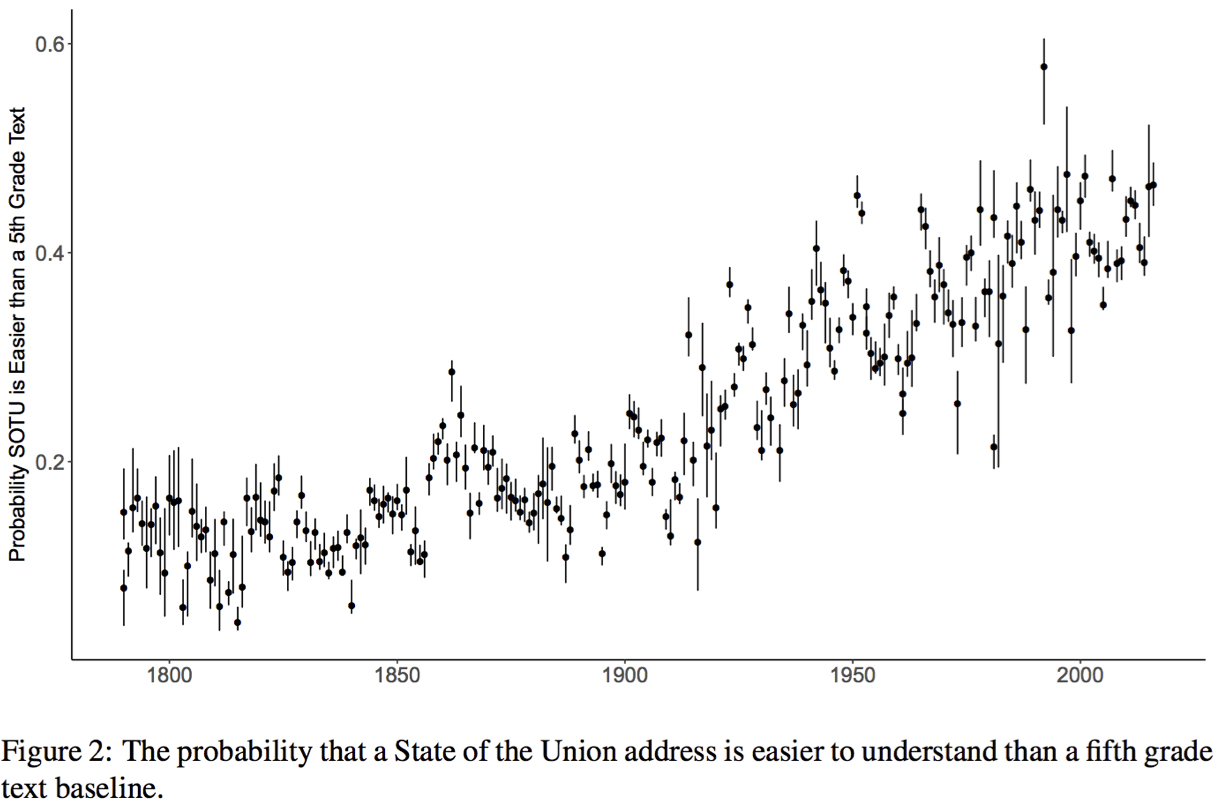
\includegraphics[height=2.8in]{Images/fig7}
%\end{centering}
%\end{figure}
%\begin{center}
%\vspace{-10pt}
% Benoit, Munger \& Spirling (2017)  
%\end{center}
%\end{frame}
%
%\begin{frame}{Example of descriptive text analysis: ideological scaling}
%\begin{figure}[h]
%\begin{centering}
%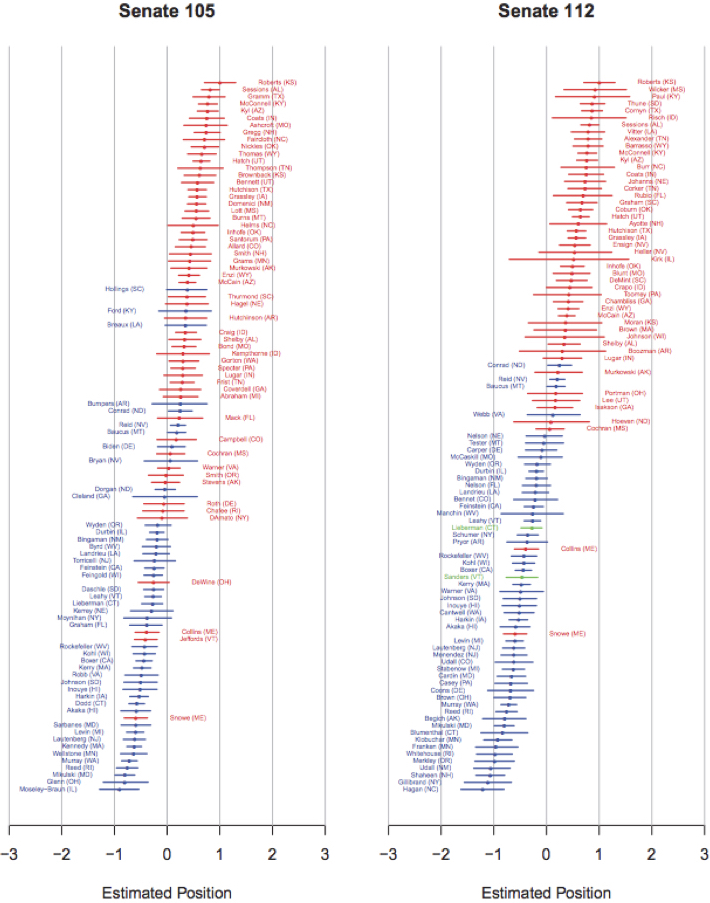
\includegraphics[height=2.9in]{Images/fig8}
%\end{centering}
%\end{figure}
%\begin{center}
%Lauderdale \& Herzog (2016)
%\end{center}
%\end{frame}

%EndExpansion

%TCIMACRO{\TeXButton{BeginFrame}{\begin{frame}}}%
%BeginExpansion
%\begin{frame}%
%EndExpansion

\begin{frame}{Representing text as data}

\begin{itemize}
\setlength{\itemsep}{0.8em}
\item When humans read text, they interpret words in light of other words, and extract meaning from the text as a whole

\pause

\item Most methods for analyzing text ignore this complexity, and treat text as a sequence of tokens

\pause

\item A token can be one word (unigram) or several words in a row (bigrams, trigrams)

\pause

\item Example: \textcolor{blue}{The president of the United States is Donald Trump}

\item Example vector after transformation in unigrams:
\begin{equation*}
\begin{array}{cccccccc}
the & president & of & united & states & is & donald & trump \\ 
2 & 1 & 1 & 1 & 1 & 1 & 1 & 1%
\end{array}%
\end{equation*}

\item Common bigrams will be $united.states$ and $donald.trump$
\end{itemize}
\end{frame}

\begin{frame}{Pre-Processing}

\begin{itemize}
\setlength{\itemsep}{0.8em}
\item An important part of the ``art'' of text analysis is deciding what data to throw out

\item Uninformative data add noise and are computationally costly

\pause

\item Steps to reduce the number of features:

\vspace{4pt}

\begin{itemize}
\setlength{\itemsep}{0.45em}
\item Tokenization: split raw character strings into individual elements 
\pause
\item Remove non-alphabetic elements, e.g., numbers, symbols, HTML tags (careful with ``@'', ``\#'', etc.)
\pause
\item Remove punctuation (careful with ``-'' for hyphenated words)
\pause
\item Convert to lower case (caution e.g., ``US'' or ``us'')
\pause
\item Remove very common words and very rare ones
\pause
\item Stemming/lemmatizing
\end{itemize}
\end{itemize}

\end{frame}

\begin{frame}{Pre-processing : stopword removal}
\begin{itemize}
\setlength{\itemsep}{1.2em}
\item The frequency distribution of words in natural languages is highly skewed (Zipf's law), with a few dozen words accounting for the bulk of text

\item We want to eliminate very common words that are used as connectors. They take up memory but do not help distinguish one document from another

\item These are called stopwords ad include articles, conjunctions, prepositions, etc.. No definitive list, but some frequently used

\pause

\item Depending on the application one can also construct list of context- specific stop words or expressions (more below)
\end{itemize}
\end{frame}

\begin{frame}{Common English stop words}
\begin{figure}[h]
\begin{centering}
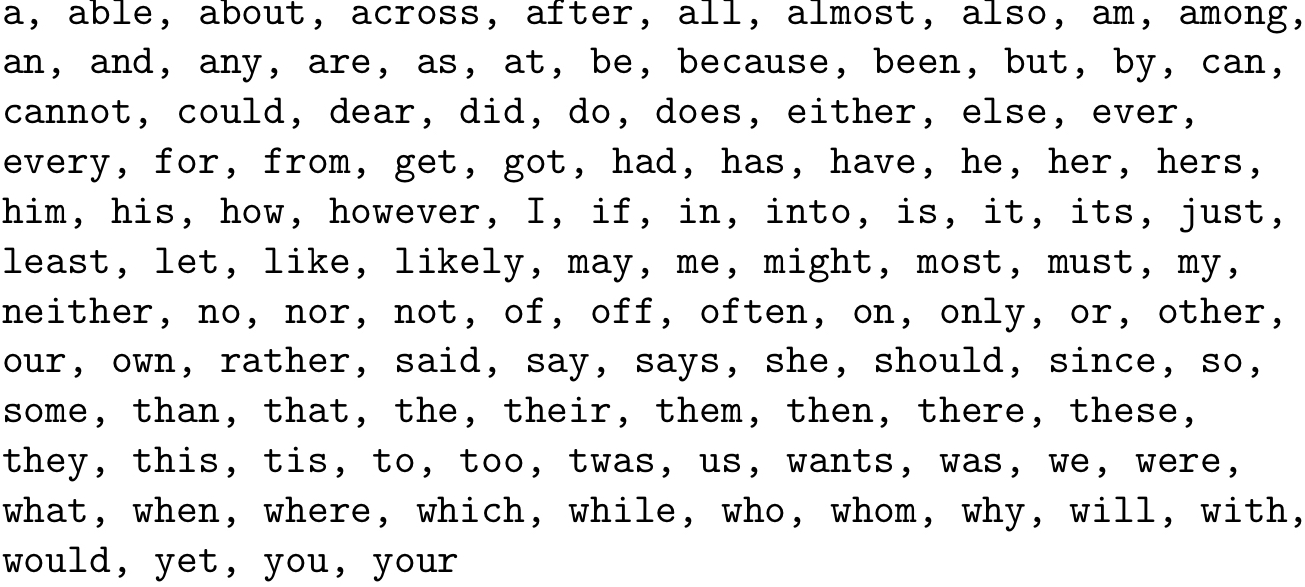
\includegraphics[height=1.9in]{Images/fig9}
\end{centering}
\end{figure}
\begin{itemize}
    \item But no list should be considered universal
\end{itemize}
\end{frame}

\begin{frame}{A more comprehensive list of stop words}
\begin{figure}[h]
\begin{centering}
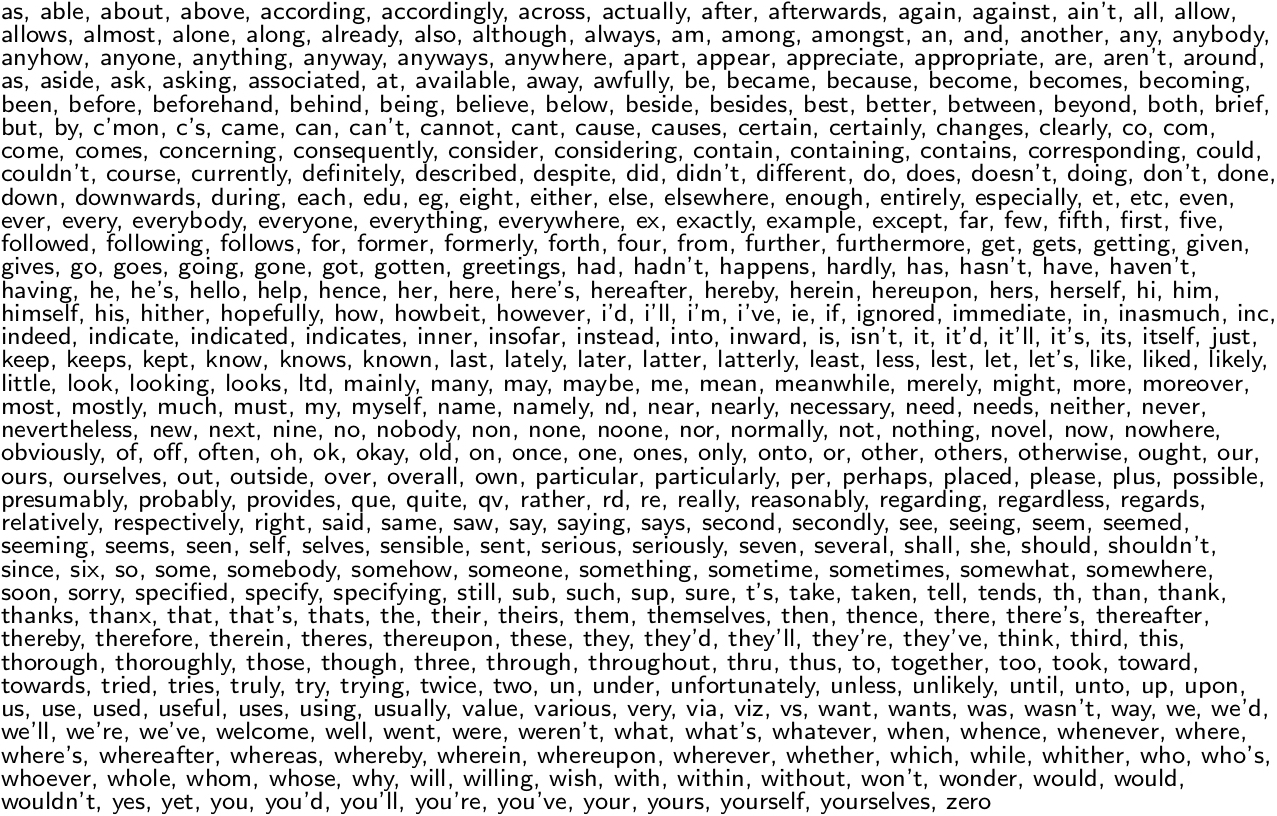
\includegraphics[height=2.8in]{Images/fig10}
\end{centering}
\end{figure}
\end{frame}

\begin{frame}{Stemming/Lemmatizing}
\begin{itemize}
\setlength{\itemsep}{1.2em}

\item Another way to reduce dimensionality is to reduce words to their common linguistic root (e.g., \textcolor{blue}{econom}y, \textcolor{blue}{econom}ics, \textcolor{blue}{econom}ically)

\pause

\item \textcolor{blue}{Stemming}: deterministic algorithm to removing suffixes (resulting stem not always a valid word). \textcolor{blue}{Porter stemmer} is popular
\vspace{5pt}
\begin{itemize}
\item Results can sometime be misleading: `university' and `universe', `policy' and `police'
\end{itemize}

\pause

\item \textcolor{blue}{Lemmatizing}: Tag each token with its part of speech, then look up each (word, POS) pair in a dictionary to find linguistic root. 
\vspace{5pt}
\begin{itemize}
\item Ex.: `saw' tagged as verb is converted to `see', `saw' tagged as noun is left unchanged.
\end{itemize}

\end{itemize}

\end{frame}

\begin{frame}{Stemming: example}
\begin{figure}[h]
\begin{centering}
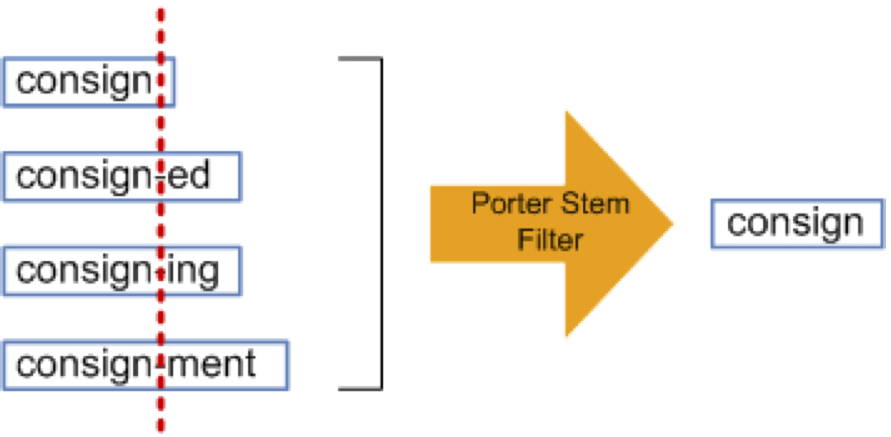
\includegraphics[height=2.15in]{Images/fig12}
\end{centering}
\end{figure}
\end{frame}

\begin{frame}{Parts of speech}
\begin{itemize}
\item The Penn ``Treebank'' is the standard scheme for tagging POS
\end{itemize}
\begin{centering}
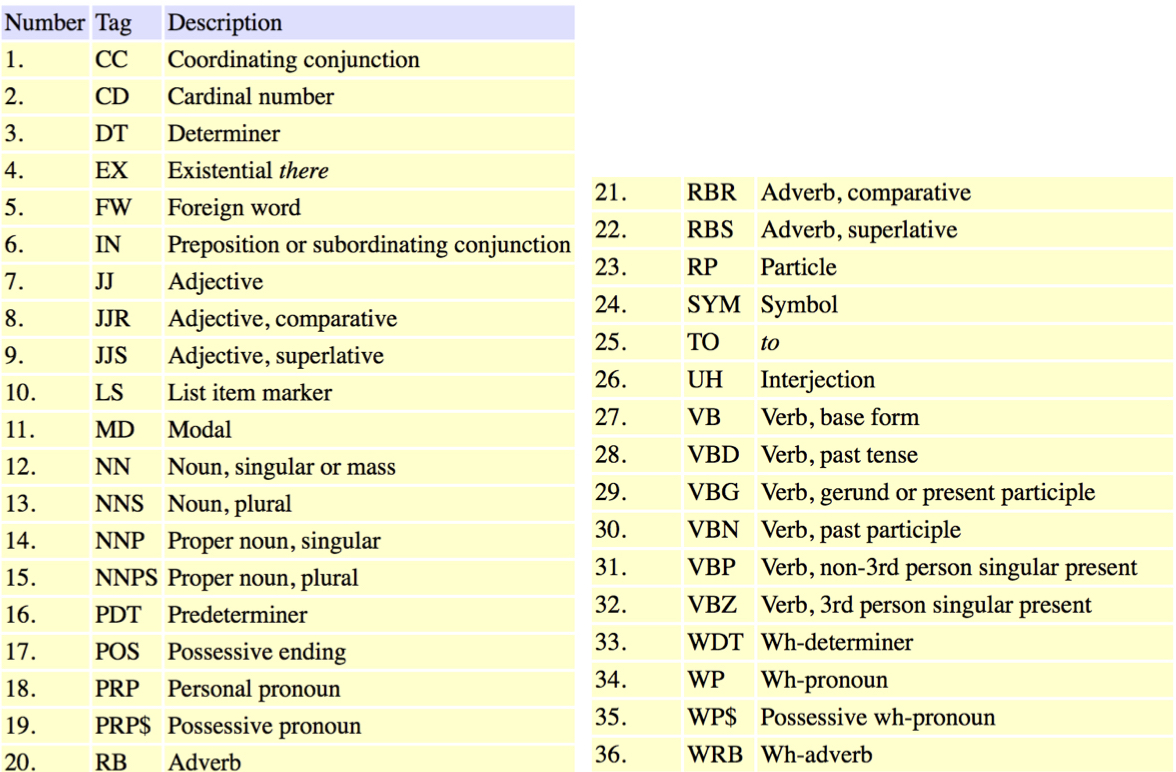
\includegraphics[height=2.8in]{Images/fig13}
\end{centering}
\end{frame}

\begin{frame}
{\normalsize{Example: NYT - March 29, 1991. Libya}}
The exiled Prince
Idris of Libya has said he will take control of a dissident Libyan
paramilitary force that was originally trained by American intelligence
advisers, and he has promised to order it into combat against Col. Muammar
el-Qaddafi, the Libyan leader. The United States' two-year effort to
destabilize Colonel Qaddafi ended in failure in December, when a
Libyan-supplied guerrilla force came to power in Chad, where the original
600 commandos were based. The new Chad Government asked the United States to
fly the Libyan dissidents out of the country, beginning a journey that has
taken them to Nigeria, Zaire and finally Kenya. So far, no country has
agreed to take them permanently. The 400 remaining commandos, who have been
disarmed, were originally members of the Libyan Army captured by Chad in
border fighting in 1988. They volunteered for the force as a way of escaping
P.O.W. camps. "Having received pledges of allegiance from leaders of the
force, Prince Idris has stepped in to assume responsibility for the troops'
welfare," said a statement released in Rome by the royalist Libyan
government in exile. It was overthrown in 1969.
\end{frame}
%
\begin{frame}
{\normalsize{Example: NYT - March 29, 1991. Libya (stopwords)}}
\textcolor{red}{the} exiled prince idris \textcolor{red}{of} libya %
\textcolor{red}{has} \textcolor{red}{said} \textcolor{red}{he} %
\textcolor{red}{will} \textcolor{red}{take} control \textcolor{red}{of} %
\textcolor{red}{a} dissident libyan paramilitary force \textcolor{red}{that} %
\textcolor{red}{was} originally trained \textcolor{red}{by} american
intelligence advisers, \textcolor{red}{and} \textcolor{red}{he} %
\textcolor{red}{has} promised \textcolor{red}{to} order \textcolor{red}{it} %
\textcolor{red}{into} combat \textcolor{red}{against} col. muammar
el-qaddafi, \textcolor{red}{the} libyan leader. \textcolor{red}{the} united
states' two-year effort \textcolor{red}{to} destabilize colonel qaddafi
ended \textcolor{red}{in} failure \textcolor{red}{in} december, %
\textcolor{red}{when} \textcolor{red}{a} libyan-supplied guerrilla force
came \textcolor{red}{to} power \textcolor{red}{in} chad, %
\textcolor{red}{where} \textcolor{red}{the} original 600 commandos %
\textcolor{red}{were} based. \textcolor{red}{the} new chad government asked %
\textcolor{red}{the} united states \textcolor{red}{to} fly %
\textcolor{red}{the} libyan dissidents \textcolor{red}{out} %
\textcolor{red}{of} \textcolor{red}{the} country, beginning %
\textcolor{red}{a} journey \textcolor{red}{that} \textcolor{red}{has} taken %
\textcolor{red}{them} \textcolor{red}{to} nigeria, zaire \textcolor{red}{and}
finally kenya. \textcolor{red}{so} far, \textcolor{red}{no} country %
\textcolor{red}{has} agreed \textcolor{red}{to} \textcolor{red}{take} %
\textcolor{red}{them} permanently. \textcolor{red}{the} 400 remaining
commandos, \textcolor{red}{who} \textcolor{red}{have} \textcolor{red}{been}
disarmed, \textcolor{red}{were} originally members \textcolor{red}{of} %
\textcolor{red}{the} libyan army captured \textcolor{red}{by} chad %
\textcolor{red}{in} border fighting \textcolor{red}{in} 1988. %
\textcolor{red}{they} volunteered \textcolor{red}{for} \textcolor{red}{the}
force \textcolor{red}{as} \textcolor{red}{a} way \textcolor{red}{of}
escaping p.o.w. camps. "having received pledges \textcolor{red}{of}
allegiance \textcolor{red}{from} leaders \textcolor{red}{of} %
\textcolor{red}{the} force, prince idris \textcolor{red}{has} stepped %
\textcolor{red}{in} \textcolor{red}{to} assume responsibility %
\textcolor{red}{for} \textcolor{red}{the} troops' welfare," %
\textcolor{red}{said} \textcolor{red}{a} statement released %
\textcolor{red}{in} rome \textcolor{red}{by} \textcolor{red}{the} royalist
libyan government \textcolor{red}{in} exile. \textcolor{red}{it} %
\textcolor{red}{was} overthrown \textcolor{red}{in} 1969.
\end{frame}

\begin{frame}
{\normalsize{Example: NYT - March 29, 1991. Libya}}
\textcolor{white}{the} exiled prince idris \textcolor{white}{of} libya %
\textcolor{white}{has} \textcolor{white}{said} \textcolor{white}{he} %
\textcolor{white}{will} \textcolor{white}{take} control \textcolor{white}{of}
\textcolor{white}{a} dissident libyan paramilitary force %
\textcolor{white}{that} \textcolor{white}{was} originally trained %
\textcolor{white}{by} american intelligence advisers, \textcolor{white}{and} %
\textcolor{white}{he} \textcolor{white}{has} promised \textcolor{white}{to}
order \textcolor{white}{it} \textcolor{white}{into} combat %
\textcolor{white}{against} col. muammar el-qaddafi, \textcolor{white}{the}
libyan leader. \textcolor{white}{the} united states' two-year effort %
\textcolor{white}{to} destabilize colonel qaddafi ended \textcolor{white}{in}
failure \textcolor{white}{in} december, \textcolor{white}{when} %
\textcolor{white}{a} libyan-supplied guerrilla force came %
\textcolor{white}{to} power \textcolor{white}{in} chad, %
\textcolor{white}{where} \textcolor{white}{the} original 600 commandos %
\textcolor{white}{were} based. \textcolor{white}{the} new chad government
asked \textcolor{white}{the} united states \textcolor{white}{to} fly %
\textcolor{white}{the} libyan dissidents \textcolor{white}{out} %
\textcolor{white}{of} \textcolor{white}{the} country, beginning %
\textcolor{white}{a} journey \textcolor{white}{that} \textcolor{white}{has}
taken \textcolor{white}{them} \textcolor{white}{to} nigeria, zaire %
\textcolor{white}{and} finally kenya. \textcolor{white}{so} far, %
\textcolor{white}{no} country \textcolor{white}{has} agreed %
\textcolor{white}{to} \textcolor{white}{take} \textcolor{white}{them}
permanently. \textcolor{white}{the} 400 remaining commandos, %
\textcolor{white}{who} \textcolor{white}{have} \textcolor{white}{been}
disarmed, \textcolor{white}{were} originally members \textcolor{white}{of} %
\textcolor{white}{the} libyan army captured \textcolor{white}{by} chad %
\textcolor{white}{in} border fighting \textcolor{white}{in} 1988. %
\textcolor{white}{they} volunteered \textcolor{white}{for} %
\textcolor{white}{the} force \textcolor{white}{as} \textcolor{white}{a} way %
\textcolor{white}{of} escaping p.o.w. camps. "having received pledges %
\textcolor{white}{of} allegiance \textcolor{white}{from} leaders %
\textcolor{white}{of} \textcolor{white}{the} force, prince idris %
\textcolor{white}{has} stepped \textcolor{white}{in} \textcolor{white}{to}
assume responsibility \textcolor{white}{for} \textcolor{white}{the} troops'
welfare," \textcolor{white}{said} \textcolor{white}{a} statement released %
\textcolor{white}{in} rome \textcolor{white}{by} \textcolor{white}{the}
royalist libyan government \textcolor{white}{in} exile. \textcolor{white}{it}
\textcolor{white}{was} overthrown \textcolor{white}{in} 1969.
\end{frame}
%
\begin{frame}
{\normalsize{Example: NYT - March 29, 1991. Libya (lemmatizing)}}
\textcolor{white}{the} exil\textcolor{red}{ed} princ\textcolor{red}{e} idri%
\textcolor{red}{s} \textcolor{white}{of} libya \textcolor{white}{has} %
\textcolor{white}{said} \textcolor{white}{he} \textcolor{white}{will} %
\textcolor{white}{take} control \textcolor{white}{of} \textcolor{white}{a}
dissid\textcolor{red}{ent} libyan paramilitar\textcolor{red}{y} forc%
\textcolor{red}{e} \textcolor{white}{that} \textcolor{white}{was} origin%
\textcolor{red}{ally} train\textcolor{red}{ed} \textcolor{white}{by}
american intellig\textcolor{red}{ence} advisers, \textcolor{white}{and} %
\textcolor{white}{he} \textcolor{white}{has} promis\textcolor{red}{ed} %
\textcolor{white}{to} order \textcolor{white}{it} \textcolor{white}{into}
combat \textcolor{white}{against} col. muammar el-qaddafi, %
\textcolor{white}{the} libyan leader. \textcolor{white}{the} unit state
two-year effort \textcolor{white}{to} destabil\textcolor{red}{ize} colonel
qaddafi end\textcolor{red}{ed} \textcolor{white}{in} failur\textcolor{red}{e}
\textcolor{white}{in} december, \textcolor{white}{when} \textcolor{white}{a}
libyan-suppli\textcolor{red}{ed} guerrilla forc\textcolor{red}{es} came %
\textcolor{white}{to} power \textcolor{white}{in} chad, %
\textcolor{white}{where} \textcolor{white}{the} origin 600 commando %
\textcolor{white}{were} based. \textcolor{white}{the} new chad govern%
\textcolor{red}{ment} ask\textcolor{red}{ed} \textcolor{white}{the} unit%
\textcolor{red}{ed} state\textcolor{red}{s} \textcolor{white}{to} fl%
\textcolor{red}{y} \textcolor{white}{the} libyan dissid\textcolor{red}{ents} %
\textcolor{white}{out} \textcolor{white}{of} \textcolor{white}{the} country,
begin\textcolor{red}{ning} \textcolor{white}{a} journey %
\textcolor{white}{that} \textcolor{white}{has} taken \textcolor{white}{them} %
\textcolor{white}{to} nigeria, zair\textcolor{red}{e} \textcolor{white}{and}
final\textcolor{red}{ly} kenya. \textcolor{white}{so} far, %
\textcolor{white}{no} countr\textcolor{red}{y} \textcolor{white}{has} agre%
\textcolor{red}{ed} \textcolor{white}{to} \textcolor{white}{take} %
\textcolor{white}{them} permanently. \textcolor{white}{the} 400 remain
commandos, \textcolor{white}{who} \textcolor{white}{have} %
\textcolor{white}{been} disarmed, \textcolor{white}{were} origin%
\textcolor{red}{ally} member\textcolor{red}{s} \textcolor{white}{of} %
\textcolor{white}{the} libyan arm\textcolor{red}{y} captur\textcolor{red}{ed}
\textcolor{white}{by} chad \textcolor{white}{in} border fight%
\textcolor{red}{ing} \textcolor{white}{in} 1988. \textcolor{white}{they}
volunt\textcolor{red}{eered} \textcolor{white}{for} \textcolor{white}{the}
forc\textcolor{red}{e} \textcolor{white}{as} \textcolor{white}{a} way %
\textcolor{white}{of} escap\textcolor{red}{ing} p.o.w. camps. "hav%
\textcolor{red}{ing} receiv\textcolor{red}{ed} pledg\textcolor{red}{es} %
\textcolor{white}{of} allegi\textcolor{red}{ance} \textcolor{white}{from}
leader \textcolor{white}{of} \textcolor{white}{the} force, princ%
\textcolor{red}{e} idri\textcolor{red}{s} \textcolor{white}{has} step%
\textcolor{red}{ed} \textcolor{white}{in} \textcolor{white}{to} assum%
\textcolor{red}{e} respons\textcolor{red}{ibility} \textcolor{white}{for} %
\textcolor{white}{the} troop\textcolor{red}{'s} welfare," %
\textcolor{white}{said} \textcolor{white}{a} statement releas%
\textcolor{red}{ed} \textcolor{white}{in} rome \textcolor{white}{by} %
\textcolor{white}{the} royalist libyan govern\textcolor{red}{meant} %
\textcolor{white}{in} exile. \textcolor{white}{it} \textcolor{white}{was}
overthrown \textcolor{white}{in} 1969.
\end{frame}
%
\begin{frame}
{\normalsize{Example: NYT - March 29, 1991. Libya}}
\textcolor{white}{the} exil princ idri \textcolor{white}{of} libya %
\textcolor{white}{has} \textcolor{white}{said} \textcolor{white}{he} %
\textcolor{white}{will} \textcolor{white}{take} control \textcolor{white}{of}
\textcolor{white}{a} dissid libyan paramilitari forc \textcolor{white}{that} %
\textcolor{white}{was} origin train \textcolor{white}{by} american intellig
advisers, \textcolor{white}{and} \textcolor{white}{he} \textcolor{white}{has}
promis \textcolor{white}{to} order \textcolor{white}{it} %
\textcolor{white}{into} combat \textcolor{white}{against} col. muammar
el-qaddafi, \textcolor{white}{the} libyan leader. \textcolor{white}{the}
unit state two-year effort \textcolor{white}{to} destabil colonel qaddafi
end \textcolor{white}{in} failur \textcolor{white}{in} december, %
\textcolor{white}{when} \textcolor{white}{a} libyan-suppli guerrilla forc
came \textcolor{white}{to} power \textcolor{white}{in} chad, %
\textcolor{white}{where} \textcolor{white}{the} origin 600 commando %
\textcolor{white}{were} based. \textcolor{white}{the} new chad govern ask %
\textcolor{white}{the} unit state \textcolor{white}{to} fli %
\textcolor{white}{the} libyan dissid \textcolor{white}{out} %
\textcolor{white}{of} \textcolor{white}{the} country, begin %
\textcolor{white}{a} journey \textcolor{white}{that} \textcolor{white}{has}
taken \textcolor{white}{them} \textcolor{white}{to} nigeria, zair %
\textcolor{white}{and} final kenya. \textcolor{white}{so} far, %
\textcolor{white}{no} countri \textcolor{white}{has} agre %
\textcolor{white}{to} \textcolor{white}{take} \textcolor{white}{them}
permanently. \textcolor{white}{the} 400 remain commandos, %
\textcolor{white}{who} \textcolor{white}{have} \textcolor{white}{been}
disarmed, \textcolor{white}{were} origin member \textcolor{white}{of} %
\textcolor{white}{the} libyan armi captur \textcolor{white}{by} chad %
\textcolor{white}{in} border fight \textcolor{white}{in} 1988. %
\textcolor{white}{they} volunt \textcolor{white}{for} \textcolor{white}{the}
forc \textcolor{white}{as} \textcolor{white}{a} way \textcolor{white}{of}
escap p.o.w. camps. "have receiv pledg \textcolor{white}{of} allegi %
\textcolor{white}{from} leader \textcolor{white}{of} \textcolor{white}{the}
force, princ idri \textcolor{white}{has} step \textcolor{white}{in} %
\textcolor{white}{to} assum respons \textcolor{white}{for} %
\textcolor{white}{the} troop welfare," \textcolor{white}{said} %
\textcolor{white}{a} statement releas \textcolor{white}{in} rome %
\textcolor{white}{by} \textcolor{white}{the} royalist libyan govern %
\textcolor{white}{in} exile. \textcolor{white}{it} \textcolor{white}{was}
overthrown \textcolor{white}{in} 1969.
\end{frame}

\begin{frame}{Importance and difficulty of pre-processing}

\begin{itemize}
\setlength{\itemsep}{1.2em}
\item Preparing your corpus for analysis can be tedious and very time-consuming

\item It is, however, a fundamental part of the work and your downstream results will depend on it

\item Pre-processing problems are specific to the corpus and to the question you try to address

\item Discussing ``general'' pre-processing procedures not very useful 

\pause

\item \textcolor{blue}{Important}: visually inspect your output to spot mistakes and get a ``feel'' for the text.
\end{itemize}

\end{frame}

\begin{frame}{Result of pre-processing}

\begin{itemize}
\setlength{\itemsep}{1.2em}
\item After pre-processing each document is a finite list of features

\item A basic representation of a corpus is the following:
\vspace{4pt}
\begin{itemize}
\setlength{\itemsep}{0.7em}

\item Index each unique feature in the corpus by some $j\in \left\{
1,...,J\right\} $, where $J$ is the number of unique terms

\item For each document $i\in \left\{ 1,...,I\right\} $ compute the count $%
c_{i,j}$ as the number of occurrences of feature $j$ in document $i$
\end{itemize}

\item The $I\times J$ matrix $C$ of all such counts is the document-term matrix

\item This representation is called the ``Bag-of-Words'' (BoW) approach

\item Largely ignores interdependence between words and``context''. Always with the goal of dimension reduction


\end{itemize}
\end{frame}

\begin{frame}{Document-term matrix}
\begin{itemize}
\setlength{\itemsep}{1.2em}
\item Example of DTM for $I$ documents and $J$ unique terms:
\end{itemize}
\begin{align*}
%\begin{bmatrix}
%\hat{X_1}\\
%\hat{X_2}\\
%...\\
%\hat{X_m}\\
%\end{bmatrix} \Leftarrow    
C = \begin{bmatrix}
c_{11} & c_{12} & ... & c_{1J} \\
c_{21} & c_{22} & ... & c_{2J} \\
\vdots & \vdots & \vdots & \vdots\\
c_{I1} & c_{I2} & ... & c_{IJ} \\
\end{bmatrix}
\end{align*}
\end{frame}

\begin{frame}{N-grams}

\begin{itemize}
\setlength{\itemindent}{-0.8em}
\setlength{\itemsep}{0.9em}
\item In some cases it may be useful to encode a limited amount of\\
\hspace{-9pt}dependence between words, considering short sentences
\item Two- or three-word sentences \textcolor{blue}{(bigrams, trigrams)} can be very\\
\hspace{-8pt}informative
\item E.g.,  \textcolor{blue}{``capital gain''},  \textcolor{blue}{``illegal aliens''},  \textcolor{blue}{``tax break''},  \textcolor{blue}{``war on terror''}
\item How to detect good candidates? Co-appearances occurring in the\\
\hspace{-8pt}data more than by chance  (e.g., $\chi^2$, mutual information measures)
\item Dimension increases exponentially with the size of phrases tracked,\\
\hspace{-8pt}but return may be small
\item Good practice: start with unigrams then evaluate  whether to extend

\end{itemize}
\end{frame}

\begin{frame}{Identify collocations: example}
\begin{figure}[h]
\begin{centering}
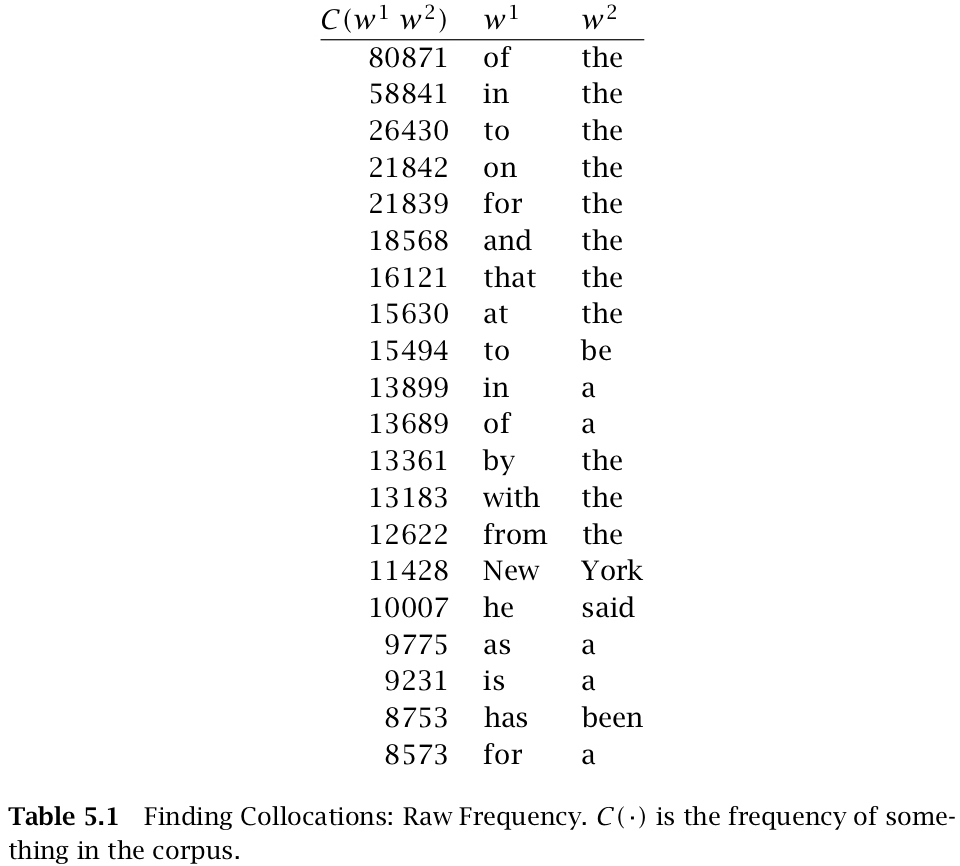
\includegraphics[height=3in]{Images/fig15}
\end{centering}
\end{figure}
\begin{center}
source: Manning and Sch\"{u}tze, \textit{FSNLP}, Ch. 5
\end{center}
\end{frame}

\begin{frame}{Identify collocations: example (cont.)}
\begin{figure}[h]
\begin{centering}
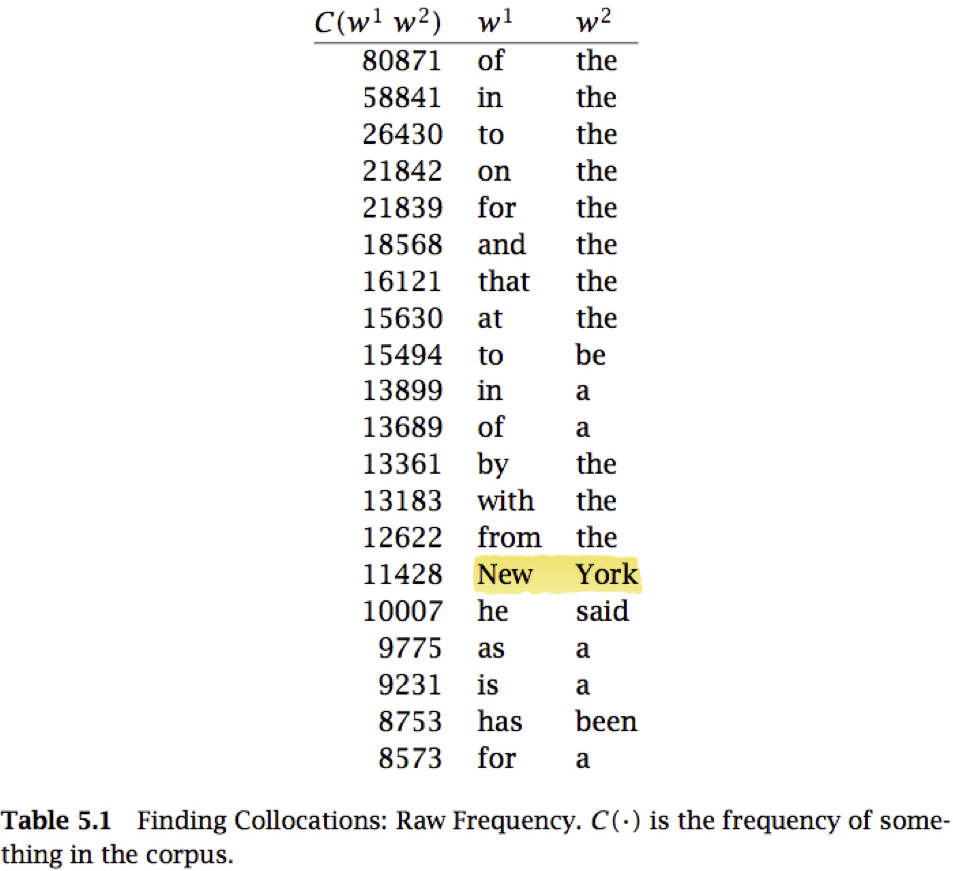
\includegraphics[height=3in]{Images/fig16}
\end{centering}
\end{figure}
\begin{center}
source: Manning and Sch\"{u}tze, \textit{FSNLP}, Ch. 5
%    \item The key is to distinguish \true collocations" from
%uninteresting word pairs/triplets/etc, such as "of the"
\end{center}
\end{frame}

\begin{frame}{Aside: pre-processed data and interfaces}
\begin{itemize}
\setlength{\itemsep}{0.8em}
\setlength{\itemindent}{-0.7em}
\item Sometimes researchers can only access data in pre-processed format
\item E.g., Google searches: you cannot retrieve the volume of searches\\
\hspace{-7pt}for every possible expression (i.e., $c_{ij}$ not observable)
\item In other cases you do not have access to raw data, but can only\\
\hspace{-7pt}access content through interfaces (e.g., ProQuest, Factiva, etc.)
\item Even if searches can be automated, you cannot produce counts for\\
\hspace{-7pt}a very large number of features
\item What searches you decide to perform is very important and\\
\hspace{-7pt}depends on priors 
\item Also, you cannot retrieve objects that may be useful for feature\\
\hspace{-7pt}selection (e.g., words occurring at least 30 times)
\end{itemize}
\end{frame}

\begin{frame}{Using text as data}
\begin{itemize}
\setlength{\itemsep}{0.85em}
\setlength{\itemindent}{-0.6em}
\item Since the number of terms is large, matrix $C$ is high-dimensional
\item Challenge to use data for empirical work is dimension reduction
\item We need to go from $C$ to predictions of a vector of attributes $\hat{V}$ we\\
\hspace{-7pt}are interested in
\item In some cases strong prior on how to map $C$ to $\hat{V}$, e.g., focusing\\
\hspace{-7pt}on specific keywords
\item Sometimes you want to capture what issues documents talk about\\
\hspace{-7pt}(topics)
\item Or in what way they are talking about a certain object (sentiment)
\item That is when high-dimensional statistical methods are used
\end{itemize}
\end{frame}

\begin{frame}{Using text as data (cont.)}
%\begin{itemize}
%\setlength{\itemsep}{1.2em}
%\item Example of DTM for $D$ documents and $V$ unique terms
%\end{itemize}
\begin{align*}
C = \begin{bmatrix}
c_{11} & c_{12} & ... & c_{1J} \\
c_{21} & c_{22} & ... & c_{2J} \\
\vdots & \vdots & \vdots & \vdots\\
c_{I1} & c_{I2} & ... & c_{IJ} \\
\end{bmatrix}\Rightarrow
\begin{bmatrix}
\hat{V_1}\\
\hat{V_2}\\
...\\
\hat{V_I}\\
\end{bmatrix}
\end{align*}
\end{frame}

\begin{frame}{Representation and feature selection}
\begin{itemize}
\setlength{\itemsep}{0.9em}
\item In its basic representation, the DTM includes simple counts, \textcolor{blue}{$c_{ij}$}, also defined as \textcolor{blue}{term frequency ($tf_{i,j}$)}
\item We can also normalize by document length: \textcolor{blue}{$tf_ {i,j}= \frac{c _ {i,j}} {\sum_{j}c_{i,j}}$}
%
%\pause

\item But the most frequent words do not necessarily have the highest diagnostic power
\pause

\item Consider a two-document matrix:
\vspace{6pt}
\begin{center}
\begin{tabular}{c|c|c|c|c}
Term & Monetary & Fiscal  & Policy &  \dots \\ \hline
                     Document \#1 & 50 & 0 & 100 & \dots  \\ \hline
                     Document \#2 & 0 & 50 & 100   & \dots
\end{tabular}
\end{center}
\item Which term can better represent each document?
\end{itemize}
\end{frame}

\begin{frame}{TF-IDF}
\begin{itemize}
\setlength{\itemsep}{1em}
\item To discount very common words, we rescale the term-frequency by the \textcolor{blue}{inverse document frequency ($idf_j$)}
\item \textcolor{blue}{$idf_j = log (I/d_j)$}, where \textcolor{blue}{$d_j=$ $\sum_{i}$
$\mathds{1}_{[c_{i,j}>0]}$}, and \textcolor{blue}{$I$} the total number of documents in the corpus

\item Hence: \textcolor{blue}{$tf$-$idf_{j}= c_{i,j} \times$ $log(\frac{I}{\sum_{i}\mathds{1}_{[c_{i,j}>0]}})$}

\pause

\item Very rare words will have low $tf$-$idf$ because \textcolor{blue}{$tf_{i,j}$} will be low

\item Words that appear in many documents will have low $tf$-$idf$ because  \textcolor{blue}{$idf_j$} will be low

\item Words that appear frequently in a few documents but not in other are the most diagnostic 

\end{itemize}

\end{frame}

\begin{frame}{Computing the tf-idf: example}
\begin{itemize}
\setlength{\itemsep}{1em}
\item Take 100 political party manifestos, each with 1000 words. \\
The first manifesto contains 16 times the word ``environment''. \\
40 of the manifestos contain the word ``environment''
\item The \textit{term frequency} is 16
\item The \textit{document frequency} is $log(100/40)=log(2.5)=0.398$
\item The \textit{tf-idf} is : $16\times 0.398 =6.368$
\item If the word appeared in 15 of the 100 manifestos, the \textit{tf-idf} would be: $16\times log(100/15)=16\times 0.824 = 13.184$ (more than twice)
\item High tf-idf is reached by a high term frequency (in a given document) and a low document frequency (in the whole corpus)
\end{itemize}
\end{frame}

\begin{frame}{TF-IDF for feature selection: data-driven stopwords}
\begin{itemize}
\setlength{\itemsep}{1.1em}
\item TF-IDF can be used to identify non-informative terms that can be classified as corpus-specific stopwords
\item Example: law, lawyer, defendant, will be very frequent in court proceedings
\item We can compute tf-idf for each term and drop words below a certain threshold
\item TF-IDF can also be used to weight features, and adapted for very cool applications (e.g., Kelly et al., 2020 paper on patents)

\end{itemize}
\end{frame}

\begin{frame}{TF-IDF for feature selection: data-driven stopwords}
\begin{itemize}
\setlength{\itemsep}{0.5\baselineskip}
    \item Example: Hansen et al. (QJE, 2017)
    \item By tf-idf adjustment, reduce unique terms from 15,394 to 8,206
\end{itemize}

\begin{center}
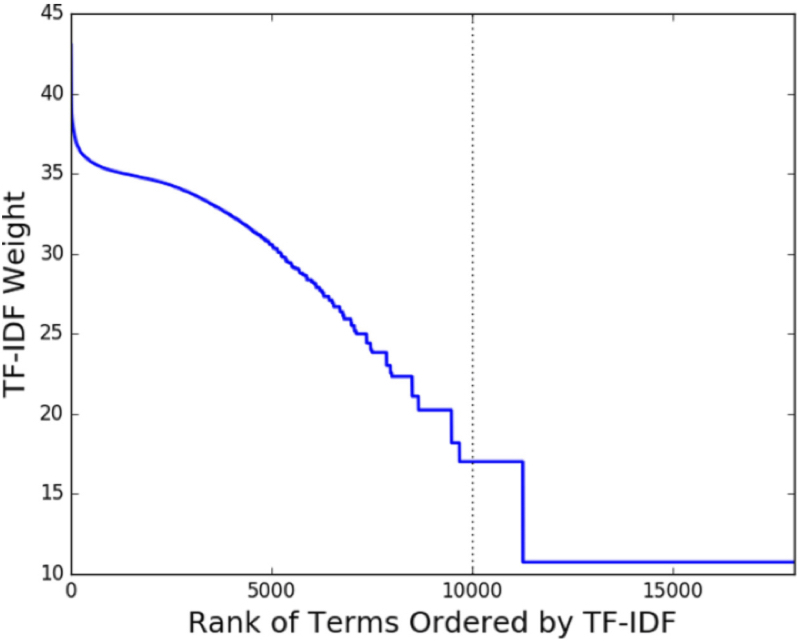
\includegraphics[height=2.5in]{Images/fig17}
\end{center}
\end{frame}


\begin{frame}{Warning and advice}

\begin{itemize}
\setlength{\itemsep}{1em}

\item You will need to take a lot of decisions when doing text mining that we will not discuss.

\item Some general advice:

\vspace{8pt}

\begin{itemize}
\setlength{\itemsep}{1em}
\setlength{\itemindent}{-0.8em}
\item Apparently silly details can have a huge impact on your measure

\item Try simple things first, look at the text, develop a ``feel'' for it

\item Think about the problem you face and what you need

\item Follow best practices but not blindly

\item At important junctions, try both ways if you have time
\end{itemize}
\end{itemize}
\end{frame}

\begin{frame}{Methods overview}
\begin{itemize}
\setlength{\itemsep}{1em}
\item There are several methods to  map word counts $C$ to some attributes $\hat{V}$
%\item Can be classified into four categories \small{(see Gentzkow et al. 2019)}:
\vspace{7pt}

\pause

\begin{enumerate}
\setlength{\itemsep}{1em}
\setlength{\itemindent}{-0.8em}
\item \textcolor{blue}{Dictionary-based methods}: do not involve statistical inference at all.\\
\hspace{-7pt}Assume $Y = f (X)$ for some known function $f(\cdot)$, E.g., presence or\\
\hspace{-7pt}number of a given term, or terms in a dictionary

\pause

\item\textcolor{blue}{Supervised methods}: observe the true value of $\hat{Y}$ for some subset\\
\hspace{-7pt}of documents (training set). The goal is to form $\hat{Y}$ for remaining\\
\hspace{-7pt}cases where Y is unobserved

\begin{itemize}
\setlength{\itemindent}{-1.5em}
\item E.g., we have a sample of emails that have been hand-coded as spam\\
\hspace{-13pt}or not spam, and want to filter new incoming emails
 \end{itemize}
 
 \pause

 \item\textcolor{blue}{Unsupervised methods}: $Y$ is unobserved; make assumptions that\\
\hspace{-7pt}allow us to infer $Y$ from $X$ (like structural approach)

\begin{itemize}
\setlength{\itemsep}{0.5em}
\setlength{\itemindent}{-1.5em}
\item E.g., principal component analysis
\item $Y$ is topic of an article; assume all articles on a given day come from\\
\hspace{-13pt}some finite set of topics; group articles based on correlation in words
\end{itemize}
 
%\item \textcolor{blue}{Text regression}: regress known features $X$ on counts of words in $D$\\
%\hspace{-7pt}to generate a model $p(X\mid D)$
%\item \textcolor{blue}{Generative models}: similar to structural model in economics, use a\\
%\hspace{-7pt}model of $p(D\mid X)$ to generate $\hat{X}$ (observed or latent features)
%\item \textcolor{blue}{Word embeddings}: based on richer representation of the underlying\\
%\hspace{-7pt}text than the token counts, allows using grammar
\end{enumerate}
\end{itemize}
\end{frame}

\begin{frame}{Methods overview: supervised methods}
\begin{itemize}
\setlength{\itemsep}{1em}
\item These come in two flavors:
\vspace{7pt}

\begin{enumerate}
\setlength{\itemsep}{1em}
\setlength{\itemindent}{-0.8em}
\item \textcolor{blue}{Regressions}: methods for linear or non-linear regression of $Y$ on\\
\hspace{-7pt}many RHS variables $X$

\begin{itemize}
\setlength{\itemindent}{-1.5em}
\setlength{\itemsep}{0.3em}
\item Penalized least squares and logistic regression (Lasso, Ridge, etc.)
\item Trees, forests, spike \& slab regression, etc.
\item Support Vector Machines
\item Neural Nets
\end{itemize}

\pause

\item\textcolor{blue}{Generative models}: write down an explicit model for $X$ as a function\\
\hspace{-7pt}of $Y$, then use it to derive an estimator for $Y$ from $X$

\begin{itemize}
\setlength{\itemindent}{-1.5em}
\setlength{\itemsep}{0.3em}
\item Naive Bayes
\item Partial Least Squares
\item Multinomial Inverse Regression (Taddy 2013)
\end{itemize}

\end{enumerate}
\end{itemize}
\end{frame}

\begin{frame}{Methods overview: unsupervised methods}
\begin{itemize}
\setlength{\itemsep}{1em}
\item These \textit{\textbf{must}} involve generative models
\item\textcolor{blue}{Examples}:
\vspace{4pt}
\begin{itemize}
\setlength{\itemindent}{-1.5em}
\setlength{\itemsep}{0.3em}
\item Principal components
\item K-means clustering
\item Topic models
\end{itemize}
\end{itemize}
\end{frame}

%\begin{frame}{Methods overview}
%\begin{itemize}
%\setlength{\itemsep}{1em}
%\item There are several methods to  map word counts $C$ to some attributes $\hat{V}$
%\item Can be classified into four categories \small{(see Gentzkow et al. 2019)}:
%\vspace{10pt}
%
%\begin{enumerate}
%\setlength{\itemsep}{1em}
%\setlength{\itemindent}{-0.8em}
%\item \textcolor{blue}{Dictionary-based methods}: do not involve statistical inference at all.\\
%\hspace{-7pt}Some terms are counted depending on a dictionary
%\item \textcolor{blue}{Text regression}: regress known features $X$ on counts of words in $D$\\
%\hspace{-7pt}to generate a model $p(X\mid D)$
%\item \textcolor{blue}{Generative models}: similar to structural model in economics, use a\\
%\hspace{-7pt}model of $p(D\mid X)$ to generate $\hat{X}$ (observed or latent features)
%\item \textcolor{blue}{Word embeddings}: based on richer representation of the underlying\\
%\hspace{-7pt}text than the token counts, allows using grammar
%\end{enumerate}
%\end{itemize}
%\end{frame}

\begin{frame}{Simple but interesting document attributes}

\begin{itemize}
\setlength{\itemsep}{1em}
\setlength{\itemindent}{-0.5em}
\item Several basic attributes of documents can be of interest to the\\
\hspace{-5pt}researcher:
\vspace{12pt}
\begin{itemize}
\setlength{\itemsep}{1.5em}
\setlength{\itemindent}{-1em}
\item \textcolor{blue}{Length}: in characters, words, lines, sentences, paragraphs, pages, etc.
\item \textcolor{blue}{Readability}: length of sentences/words, simple vs. complex words
\item \textcolor{blue}{Vocabulary diversity:} \# of unique words used over total words used
\end{itemize}
\end{itemize}
\end{frame}

\begin{frame}{Number and length of documents}
\begin{itemize}
\setlength{\itemsep}{1.2em}
\setlength{\itemindent}{-0.5em}
\item The number and the length of documents already provide interesting variables for analysis
\item For example:
\vspace{5pt}
\begin{itemize}
\setlength{\itemsep}{1.5em}
\setlength{\itemindent}{-1.3em}
\item How do electoral incentives and aging affect judges' effort and writing\\
\hspace{-12pt}style?
\end{itemize}
\item Ash and MacLeod (2015, 2017):
\vspace{5pt}
\begin{itemize}
\setlength{\itemsep}{0.5em}
\setlength{\itemindent}{-1.3em}
\item State supreme courts: highest appellate court for each of the 50 U.S.\\
\hspace{-12pt}states
\item 1.1 million judicial opinions for 1947-1994
\end{itemize}
\end{itemize}
\end{frame}

\begin{frame}{Number and length of documents (cont.)}
\begin{itemize}
\setlength{\itemsep}{1.2em}
\setlength{\itemindent}{-0.5em}
\item Left panel: Partisan Elections - Right panel: Non-Partisan Elections
\end{itemize}
\begin{center}
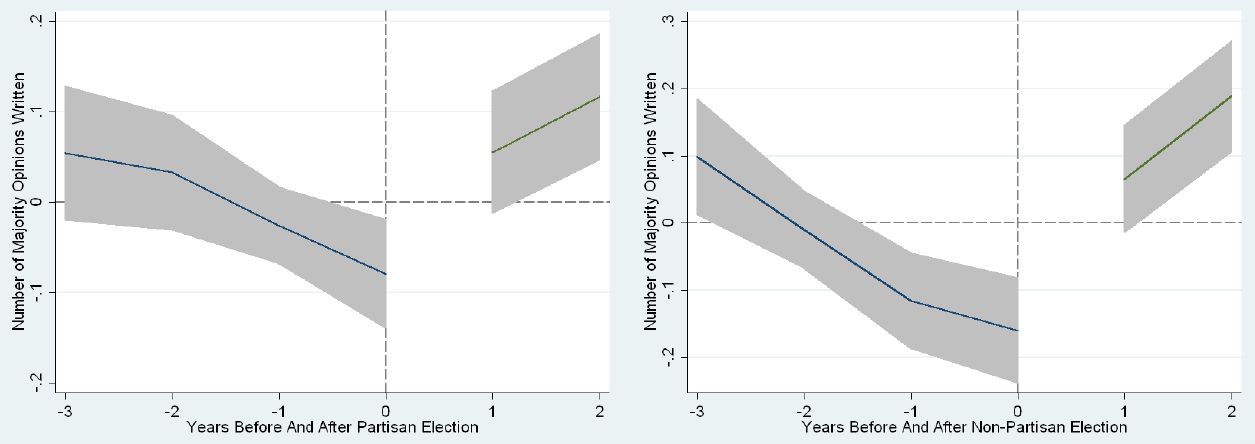
\includegraphics[scale=0.25]{Images/ash_macleod.png}
\end{center}
\begin{itemize}
\setlength{\itemsep}{1.2em}
\setlength{\itemindent}{-0.5em}
\item Elections reduce the number of opinions written
\end{itemize}
\end{frame}

\begin{frame}{Judge age distribution}
\begin{center}
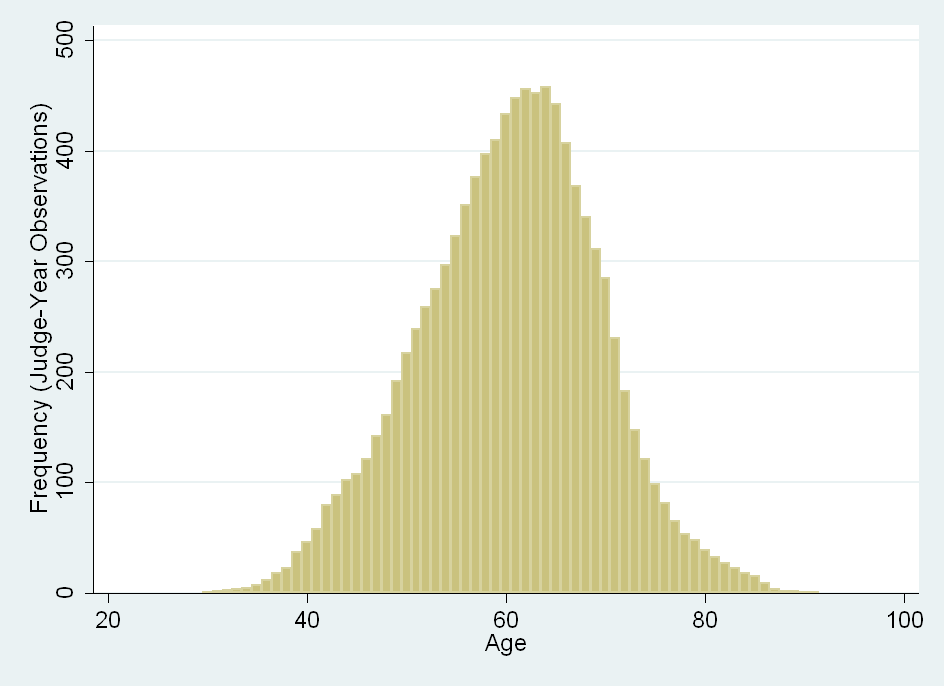
\includegraphics[scale=0.25]{Images/ash_macleod2.png}
\end{center}
\begin{itemize}
\setlength{\itemsep}{1.2em}
\setlength{\itemindent}{-0.5em}
\item State supreme court judges have a wide age range but all do the\\
\hspace{-5pt}same work task
\end{itemize}
\end{frame}

\begin{frame}{Judge age and output}
\begin{center}
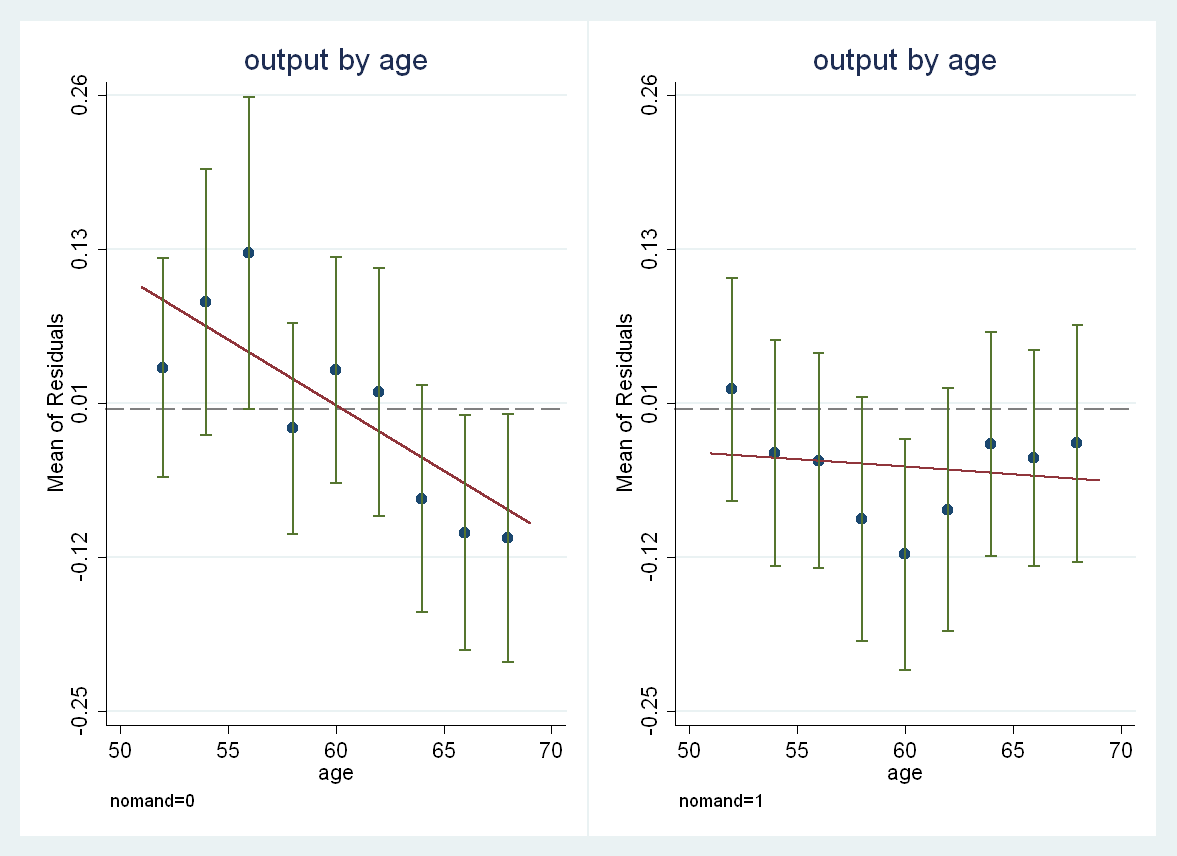
\includegraphics[scale=0.19]{Images/ash_macleod3.png}
\end{center}
\vspace{-5pt}
\begin{itemize}
\setlength{\itemsep}{0.5em}
\setlength{\itemindent}{-0.5em}
\item Judge output decreases with age, but only under mandatory\\
\hspace{-5pt}retirement (left panel)
\item Consistent with an incentive rather than physiological effect
\end{itemize}
\end{frame}

\begin{frame}{Characters-per-word and judge age}
\begin{center}
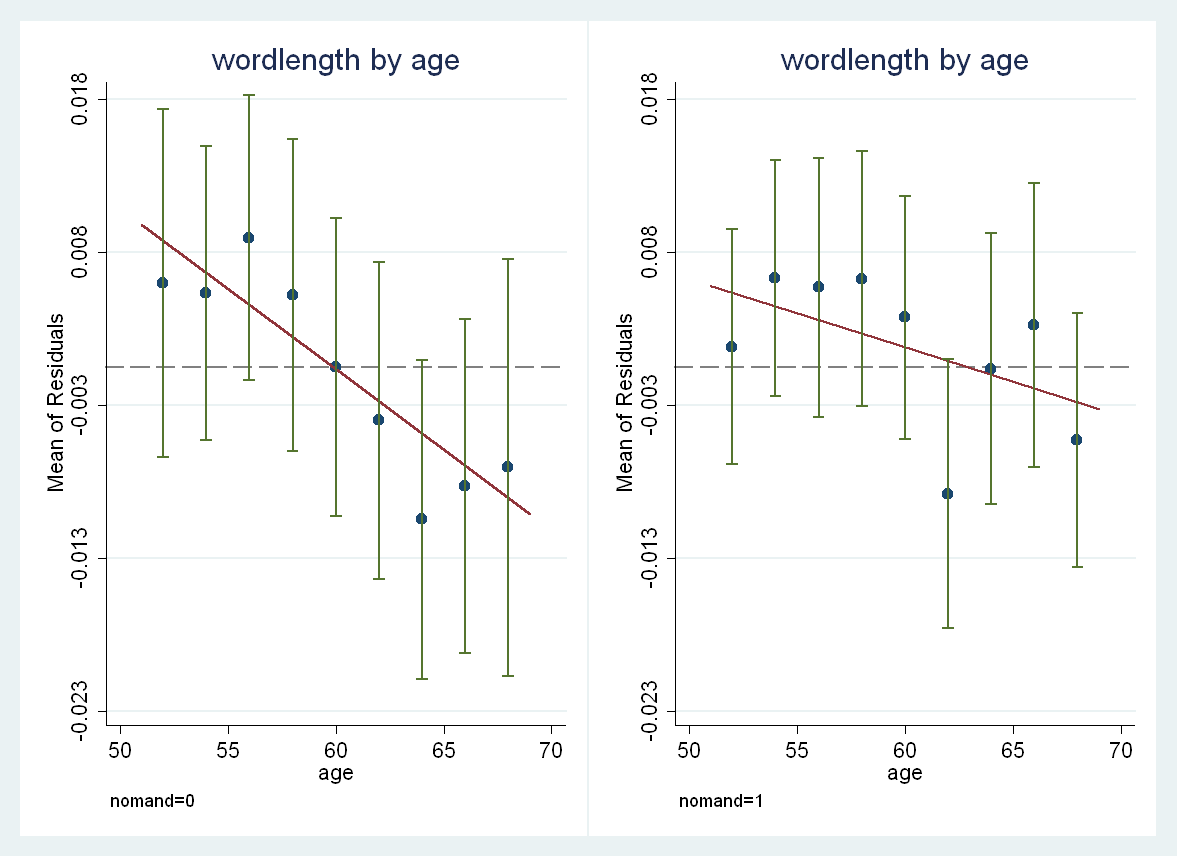
\includegraphics[scale=0.19]{Images/ash_macleod4.png}
\end{center}
\vspace{-5pt}
\begin{itemize}
\setlength{\itemsep}{0.5em}
\setlength{\itemindent}{-0.5em}
\item Older judges use shorter words (fewer characters per word)
\end{itemize}
\end{frame}

\begin{frame}{Lexical diversity}
\begin{itemize}
\setlength{\itemsep}{0.9em}
\setlength{\itemindent}{-0.5em}
\item Standard measure: \textcolor{blue}{Type-to-Token Ratio (TTR)}
\item Types: number of unique words in a document
\item Tokens: total number of words in the document
\item Problem: TTR very sensitive to overall document length, since\\
\hspace{-5pt}longer texts tend to exhibit more word repetitions
\item Alternative measures: 
\vspace{5pt}
\begin{itemize}
\setlength{\itemsep}{0.5em}
\setlength{\itemindent}{-1em}
\item \textcolor{blue}{Guiraud}: 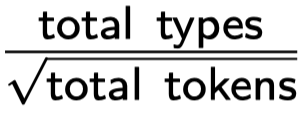
\includegraphics[scale=0.3]{Images/guiraud}
\item \textcolor{blue}{D}: randomly sample a fixed number of tokens and count the types
\end {itemize}
\end{itemize}
\end{frame}

\begin{frame}{Lexical diversity: example}
\begin{itemize}
\setlength{\itemsep}{0.5em}
\setlength{\itemindent}{-0.5em}
\item Labb\'{e} et al. (2004): study lexical diversity in a corpus of\\
\hspace{-5pt}concatenated weekly speeches by De Gaulle (1958-1969)
\item While most speeches were written, during a period in December\\
\hspace{-5pt}1965 he delivered more spontaneous press conferences
\end{itemize}

\begin{center}
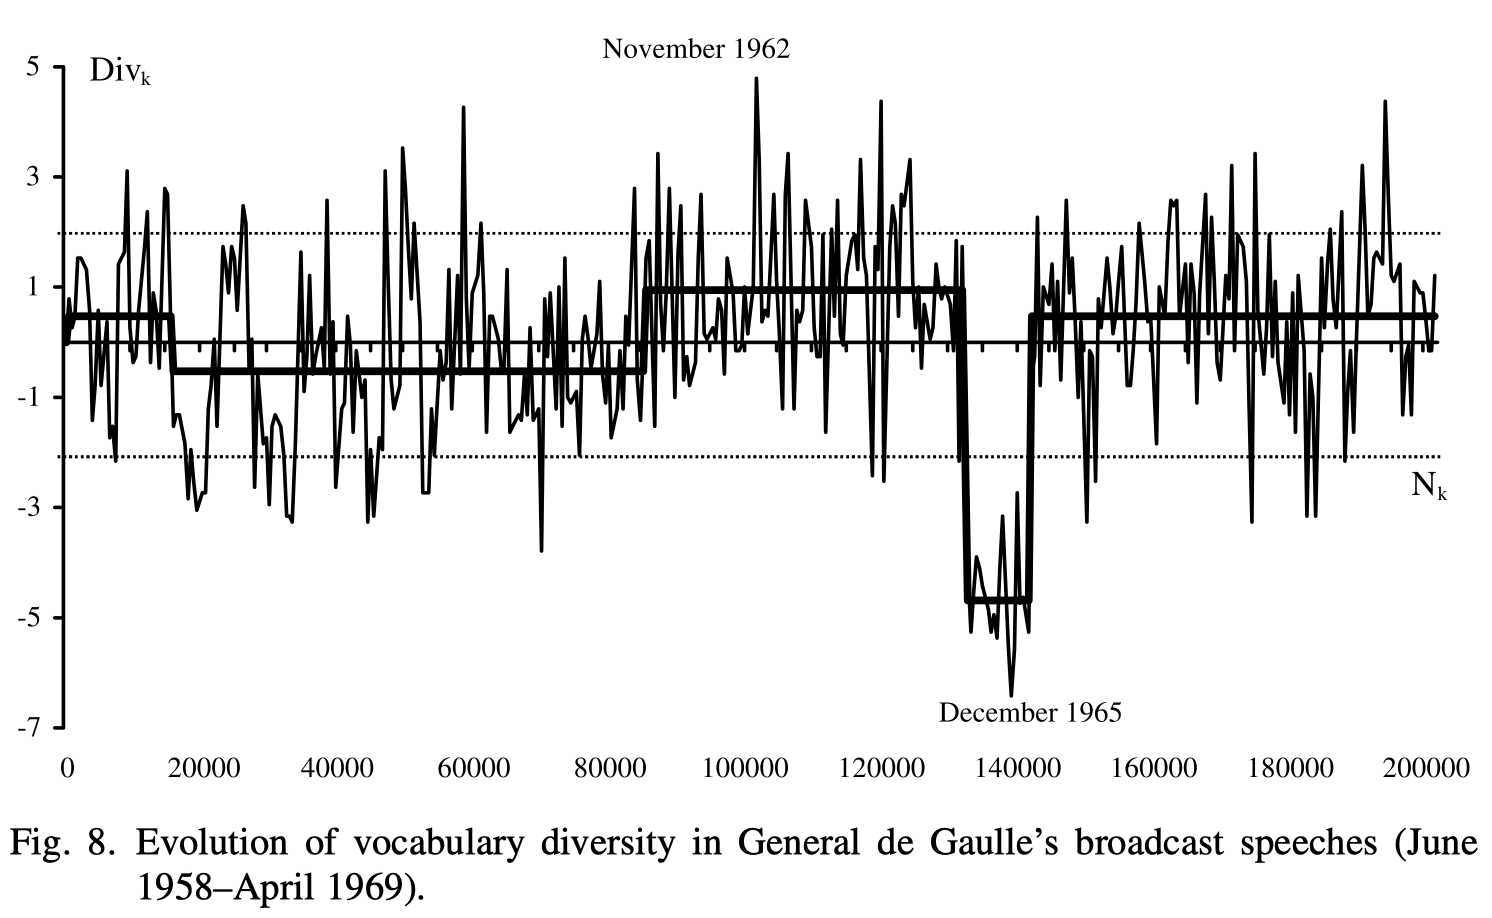
\includegraphics[scale=0.33]{Images/labbe.png}
\end{center}
\end{frame}


\begin{frame}{Complexity and readability}
\begin{itemize}
\setlength{\itemsep}{1.2em}
\setlength{\itemindent}{-0.5em}
\item Use a combination of syllables and sentence length to capture\\
\hspace{-5pt}``readability'' and ease of understanding
\item Commonly used in educational research, also applied to describe\\
\hspace{-5pt}textual complexity (e.g., political speeches)
\item No natural scale, so most are calibrated in terms of some\\
\hspace{-5pt}interpretable metric (e.g., level of education needed to understand)
\item Easily implemented in python using package \textit{textstatistics}
\end {itemize}
\end{frame}

\begin{frame}{Flesch-Kincaid readability index}
\begin{itemize}
\setlength{\itemsep}{1.3em}
\setlength{\itemindent}{-0.5em}
\item Modification of the original \textcolor{blue}{Flesch Reading Ease Index}:\\
\vspace{5pt}
\begin{center}
206.835 -1.015 $(\frac{total\:words}{total\:sentences})$ - 84.6 $(\frac{total\:syllables}{total\:words})$
\end{center}
\vspace{5pt}
\item \textcolor{blue}{Interpretation:} 0-30: university level; 60-70: understandable by a\\
\hspace{-5pt}13-15 year old; 90-100: easily understood by an 11-year old student

\item \textcolor{blue}{Flesch-Kincaid} rescaled to the U.S. educational grade levels (1-12):\\
\vspace{5pt}
\begin{center}
0.39 $(\frac{total\:words}{total\:sentences})$ + 11.8 $(\frac{total\:syllables}{total\:words}) -15.59$
\end{center}
\vspace{5pt}
\end {itemize}
\end{frame}

\begin{frame}{Politicians' language (Durante et al., AER 2019)}
\begin{itemize}
\begin{small}
\item  38 televised interventions between 1989 and 2014
\vspace{0.1cm}
\item 15 politicians, 50 hours of footage, 280,000 spoken words
\vspace{0.1cm}
\item  Measures: Gulpease index (adaptation to italian of F-K), and share of ``commonly used words'' (De Mauro-Vedovelli, 1980)
\end{small}
\end{itemize}

\begin{figure}
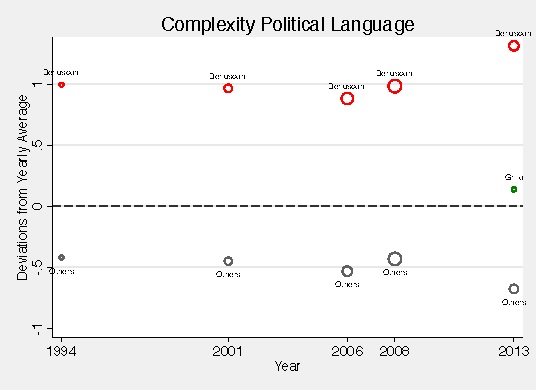
\includegraphics[scale=0.8]{Images/complexity_pol_language2.pdf}
\end{figure}

\end{frame}

\begin{frame}{Dictionary-based methods}
\begin{itemize}
\setlength{\itemsep}{1em}
\item Dictionary methods specify \textcolor{blue}{$\hat{v_i}=f (c_i)$} for some function \textcolor{blue}{$f(\cdot)$}

\end{itemize}

\vspace{12pt}

\textcolor{blue}{Examples}:

\vspace{7pt}

\begin{itemize}
\setlength{\itemsep}{1em}

\item Baker et al. (2016): use counts of specific words to generate measure of policy uncertainty

\item Tetlock (2007): applies dictionary methods to WSJ articles to generate measures of ``positive'' and ``negative'' sentiment

\item Loughran and McDonald (2011): replicate Tetlock (2007) using dictionary of terms specific to finance

\item Hassan et al (2019): build a dictionary from textbooks to measure firm-specific political risk

%\item Gentzkow and Shapiro (2010): use frequency of words in politicians' speeches and news articles to measure partisan bias

\end{itemize}
\end{frame}

\begin{frame}{Dictionary-based methods: boolean searches}
\begin{itemize}
\setlength{\itemsep}{1em}
\item Boolean searches provide a \textcolor{blue}{binary representation} of each document based on whether it includes certain terms or not
\item Define an \textit{incidence matrix} $\mathbf { X } ^ { \prime }$ where $x_{dv}'=\mathds{1} \left( x_{dv} > 0 \right)$
\item We can define Boolean expressions involving \textcolor{blue}{AND}, \textcolor{blue}{OR}, and \textcolor{blue}{NOT} on the columns of $\mathbf { X } ^ { \prime }$

\item Boolean search key to many document-retrieval systems, and built into many search engines
\vspace{8pt}

\item\textcolor{blue}{Advantage}: hard work of indexing documents has been done for you, no need to collect data yourself

\item\textcolor{blue}{Disadvantage}: can often not access raw data and produce count for very large feature sets 

\end{itemize}
\end{frame}

\begin{frame}{Economics application: Baker et al., QJE 2016}
\begin{itemize}
\setlength{\itemsep}{0.9em}
\item \textcolor{blue}{Question}: can we use data from news articles to construct a measure of economic policy uncertainty?
\item Create an index based on Boolean searches in articles from major US and European newspapers
\item For each paper on each day since 1985 submit this query:
\vspace{3pt}
\begin{itemize}
\item Article contains ``uncertain'' OR ``uncertainty'', AND
\item   Article contains ``economic'' OR ``economy'', AND 
\item  Article contains ``congress'' OR ``deficit'' OR ``federal reserve'' OR ``legislation'' OR``regulation'' OR ``white house''
\end{itemize}
\item Take resulting article counts and normalize by total newspaper articles that month. Standardize for each paper, take average across papers, normalize so that mean=100

\item Create variable that captures the \textcolor{blue}{presence} (but not the intensity) of EPU-related words in articles
\end{itemize}
\end{frame}

\begin{frame}{Results}
%\begin{figure}[h]
\begin{centering}
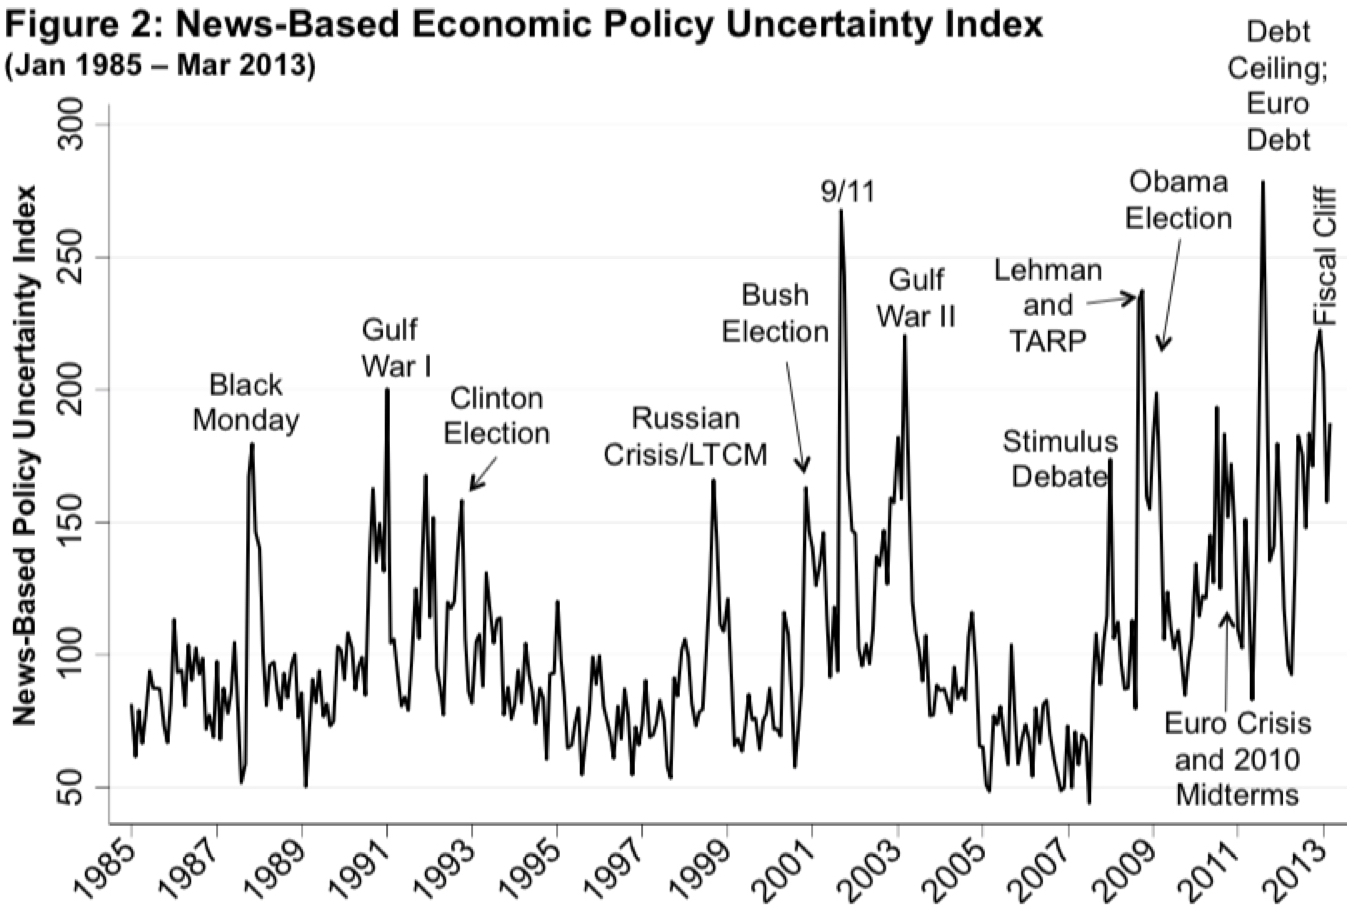
\includegraphics[height=3in]{Images/fig18}
\end{centering}
%\end{figure}
\end{frame}
%
\begin{frame}{Why using text?}
\begin{itemize}
\setlength{\itemsep}{1.2em}
\item VIX is an asset-based measure of uncertainty: implied S\&P 500 volatility at 30-day horizon using option prices
\item So what does text add to this?
\vspace{7pt}
\begin{itemize}
\setlength{\itemsep}{0.8em}
\item Focus on broader type of uncertainty besides equity prices
\item Much richer historical time series
\item Cross-country measures
\end{itemize}
\pause
\item What limitations?
\vspace{7pt}
\begin{itemize}
\setlength{\itemsep}{0.8em}
\item Choice of terms totally ad hoc
\item Dynamic of EPU index intuitive, but unclear whether this is robust to alternative choices
\end{itemize}
\end{itemize}
\end{frame}

\begin{frame}{Dictionary-based methods: word counts}
\begin{itemize}
\setlength{\itemsep}{1.3em}
\item Let $\mathfrak{D}$ be the set of keywords of interest
\item We can then represent each document $i$ as $c_{i} =\sum_ {j\in\mathfrak{D}} c_{i,j}$ or normalize, e.g. $s_ {i} = \sum_{j\in\mathcal{D}}c_{i,j} / \sum_ {i}c _{i,j}$. \\
\item This approach also considers the \textcolor{blue}{intensity} of word use to be informative
\end{itemize}
\end{frame}
%
\begin{frame}{Economic applications: Tetlock (JFE, 2007)}
\begin{itemize}
\setlength{\itemsep}{0.8em}
\item Applies dictionary methods to the Wall Street Journal's ``Abreast of the Market'' column
\item Uses Harvard IV-4 General Inquirer dictionary
\item 77 non-mutually-exclusive nor exhaustive categories: positive, negative, weak, fail, fall, pain, pleasure, rituals, etc.
\item Count number of words in each category for each column published between 1984 and 1999
\item Principal components analysis shows most variation on dimensions that reflect pessimism: negative, weak, fail, fall.
\item \textcolor{blue}{Main finding}: pessimism predicts low short-term returns (measured with the Dow Jones index) followed by reversion
\end{itemize}
\end{frame}

\begin{frame}{Economic applications: Tetlock (JFE, 2007)}
\begin{center}
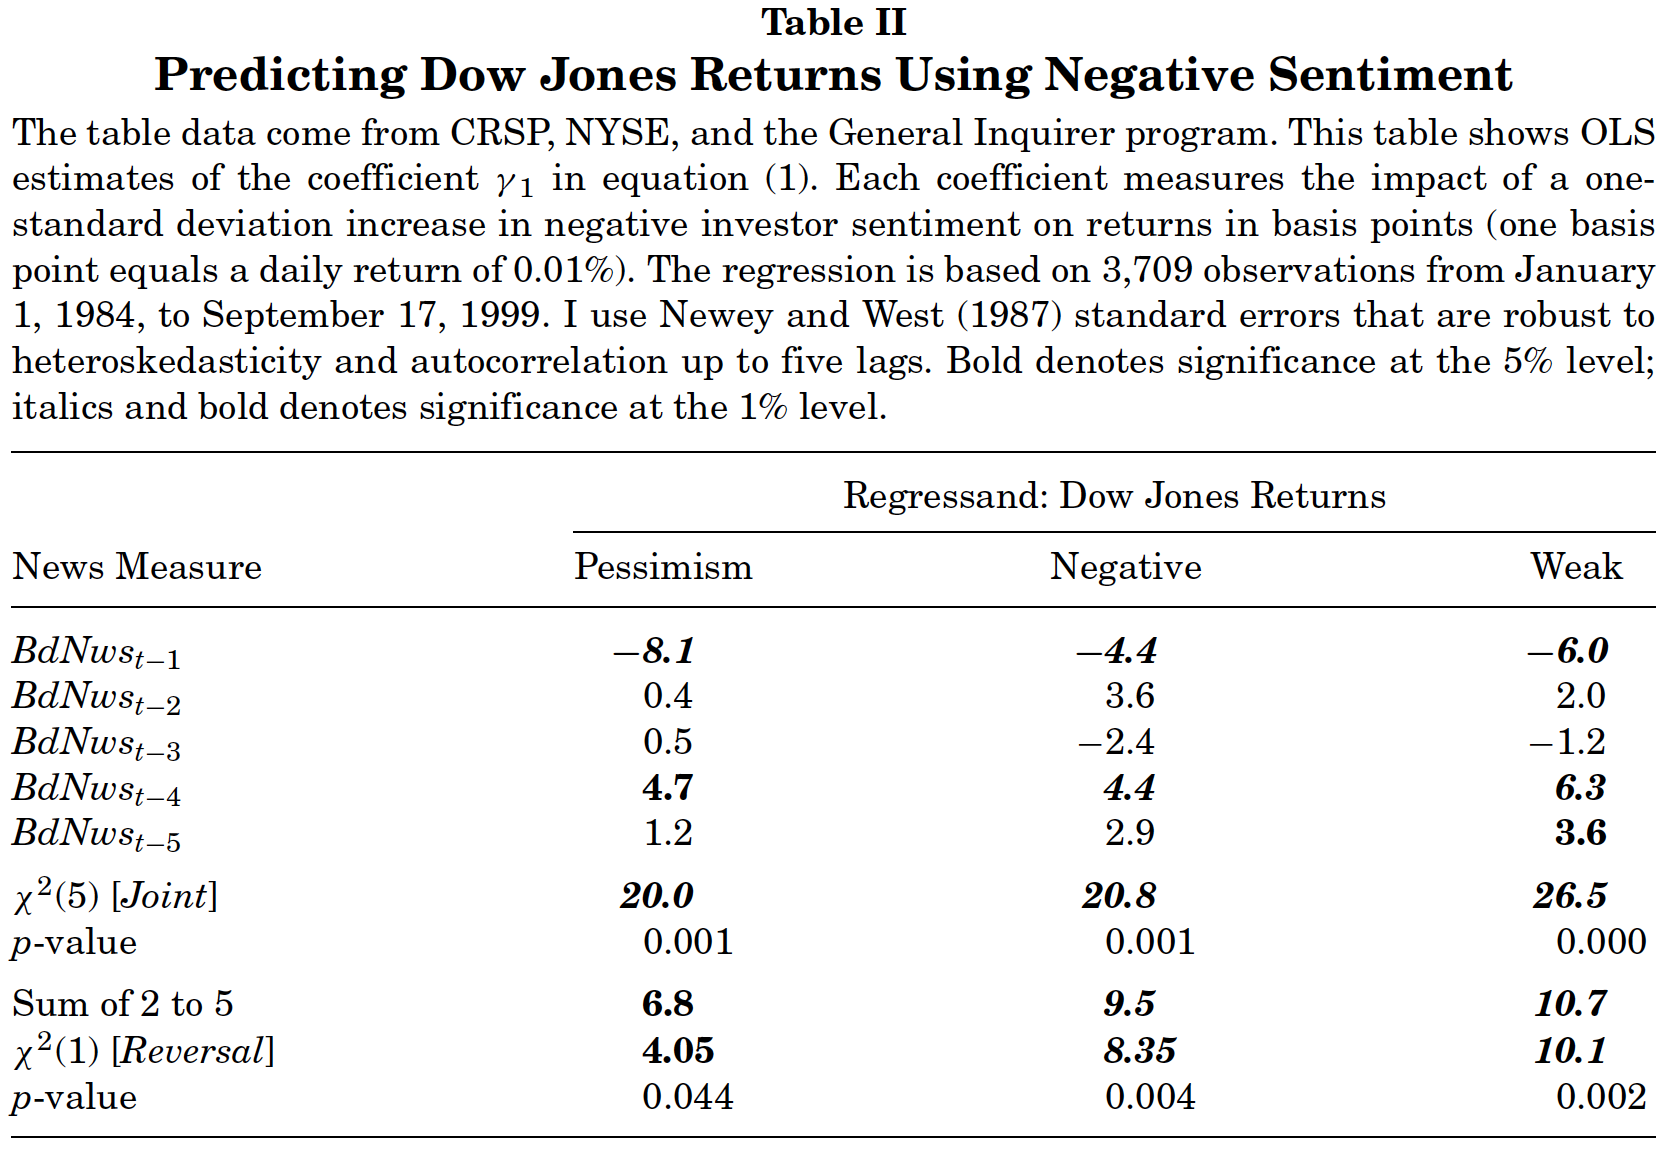
\includegraphics[scale=0.37]{Images/tetlock_fig2.png}
\end{center}
\end{frame}

\begin{frame}{Loughran and McDonald (JFE, 2011)}
\begin{itemize}
\setlength{\itemsep}{1.2em}
\item Following Tetlock (2007), popular to use just negative word dictionary from Harvard IV-4
\item This includes words like `tax', `cost', `capital', `liability', and `vice'
\item Unclear that these are appropriate for describing negative content in financial context.
\item Use 10-K filings to define their own finance-specific word lists
\item Negative list includes words like `restated', `litigation', `termination', `unpaid',`investigation', etc.
\item \textit{``Almost three-fourths of the words identified as negative by the Harvard IV-4 are typically not considered negative in financial contexts''}
\end{itemize}
\end{frame}


\begin{frame}{Loughran and McDonald (JFE, 2011)}
\begin{center}
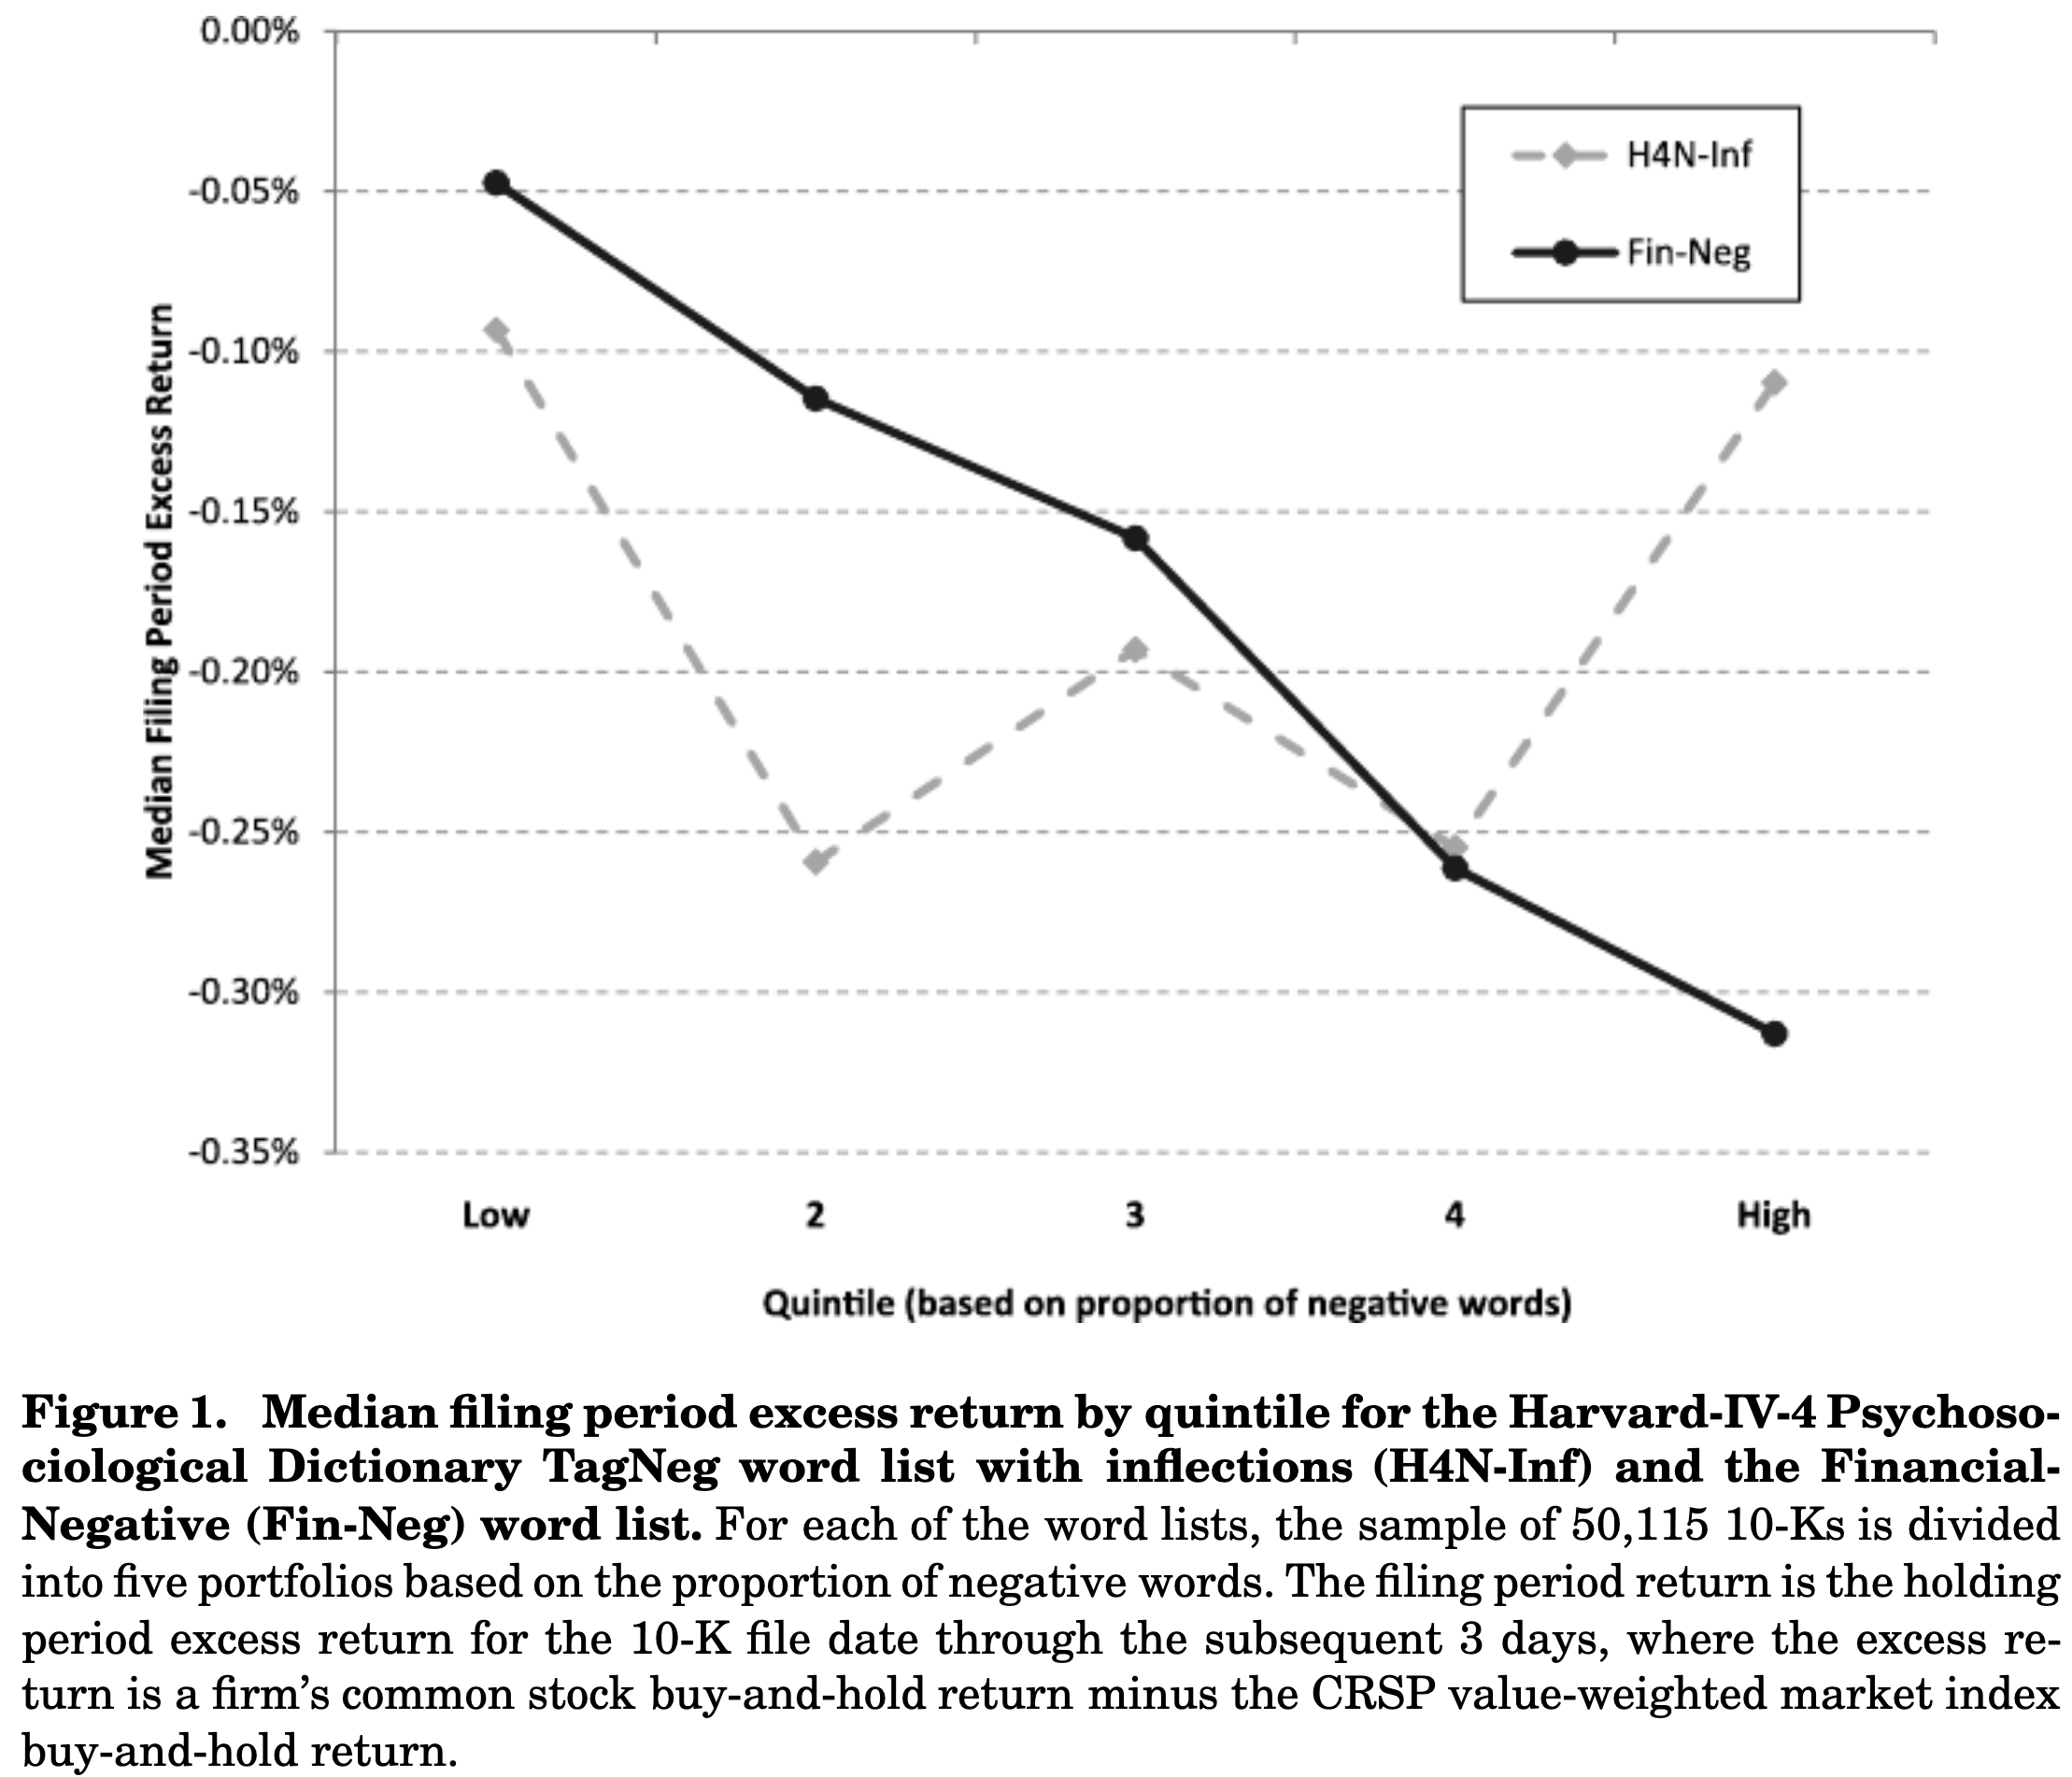
\includegraphics[scale=0.2]{Images/mcdonald_2011.png}
\end{center}

\begin{itemize}
\item \textcolor{blue}{Main finding}: context-specific dictionary has greater predictive power for return regressions than the generic one
\end{itemize}


\end{frame}

%almost three-fourths of the wordsidentified as negative by the widely used Harvard Dictionary are words typically notconsidered negative in financial contexts.

\begin{frame}{Hassan et al. (QJE, 2019): firm-level political risk}
\begin{itemize}
\setlength{\itemsep}{1.2em}
\item Another example of application of dictionary methods
\item But the construction and the use of the dictionary is innovative
\item Goal: to construct a measure of political risk faced by individual US firms
\item Data: 178,173 transcripts of quarterly earnings conference calls
\item Idea: measure the share of the conversations between call participants and firm management centered around risks associated with political matters
\end{itemize}
\end{frame}

\begin{frame}{Hassan et al. (QJE, 2019): constructing the dictionary}
\begin{itemize}
\setlength{\itemsep}{0.9em}
\item Training library of political text archetypical of discussions of political topics, $\mathbf{P}$
\item Training library of non-political text, archetypical of discussion of non-political topics, $\mathbf{N}$
\item $\mathbf{P}$: William T. Bianco and David T. Canon, \textit{American Politics Today}
\item $\mathbf{N}$: Robert Libby, Patricia A. Libby, and Daniel G. Short's, \textit{Financial Accounting}
\item Each library is the set of all adjacent two-word combinations (``bigrams'') contained in the text
\item $\boldsymbol{P}\backslash \boldsymbol{N}:$ terms that are in the political texts but not in the non-political text
\end{itemize}
\end{frame}

\begin{frame}{Hassan et al. (QJE, 2019): constructing the dictionary}
\begin{itemize}
\setlength{\itemsep}{1.2em}
\item First key statistics for them is $f_{b,\boldsymbol{P}}/B_{\boldsymbol{P}}$
\vspace{3pt}
\begin{itemize}
\setlength{\itemsep}{0.4em}
\item $f_{b,\boldsymbol{P}}$: frequency of bigram $b$ in the political training library
\item $B_{\boldsymbol{P}}$ is the total number of bigrams in the political training library
\item \textbf{What is this?}
\item Relative term frequency of $b$ in $P$. Similar to $tf_{d,v}$
\end{itemize}
\item Second key statistics is $\boldsymbol{1}\left[ b\in \boldsymbol{P} \backslash \boldsymbol{N}\right] $
\vspace{3pt}
\begin{itemize}
\setlength{\itemsep}{0.4em}
\item Where $\boldsymbol{1}\left[ \cdot \right] $ is an indicator function.
\item This is a particularly brutal way of doing an $idf_{b}$ across libraries. \textbf{Why?}
\item $idf_{b}$ would give more weight to terms that are "special" to library $\boldsymbol{P}$, i.e. not as frequent in $\boldsymbol{N.}$
\item Here the weight is set to 0 for all terms in $\boldsymbol{P}$ that are also in $\boldsymbol{N.}$
\end{itemize}
\end{itemize}
\end{frame}

\begin{frame}{Hassan et al. (QJE, 2019): constructing the dictionary}
\vspace{-7pt}
\begin{center}
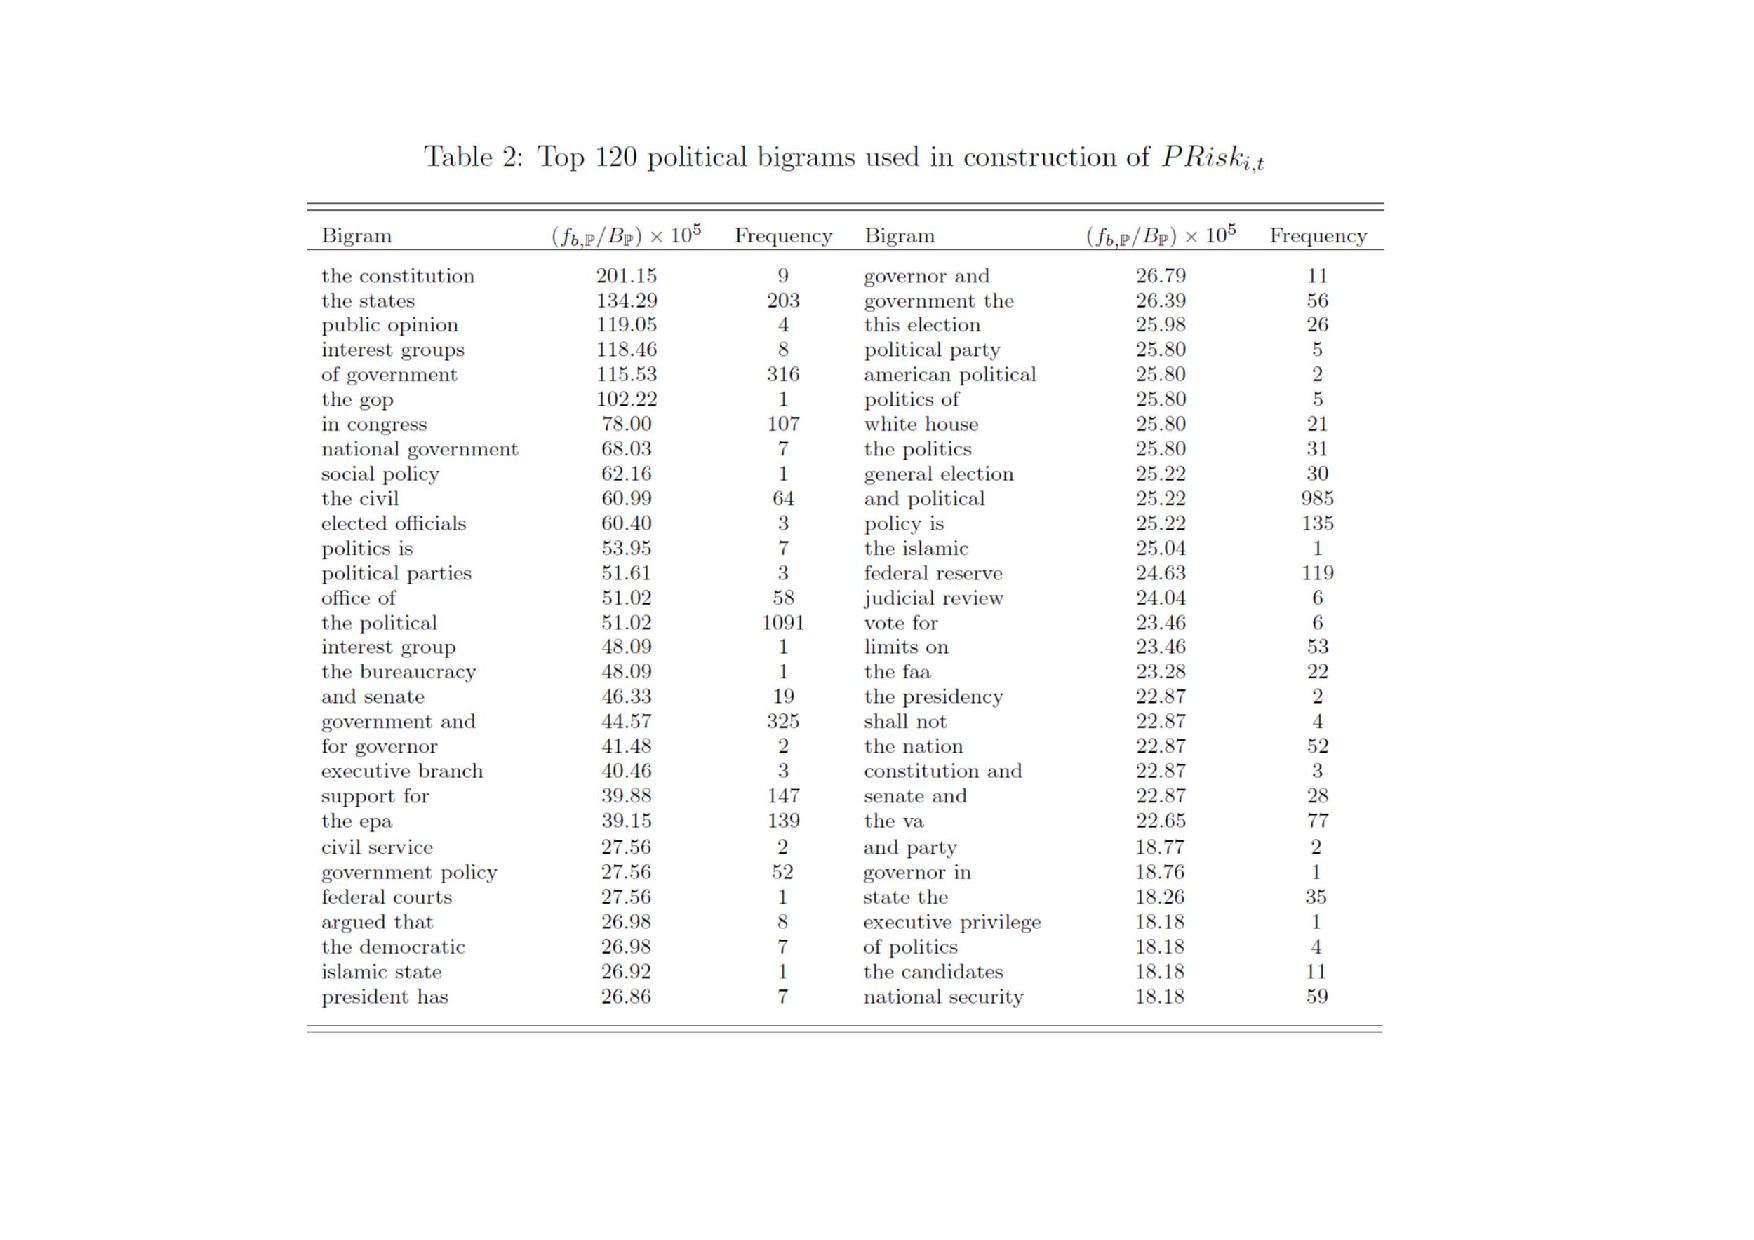
\includegraphics[scale=0.5]{Images/hassan_et_al_table1.pdf}
\end{center}
\end{frame}

\begin{frame}{Hassan et al. (QJE, 2019): using the dictionary}
\begin{itemize}
\setlength{\itemsep}{1.5em}
\item Count the number of instances where political bigrams are used in conjunction with synonyms for ``risk''
\item Conference-call transcript of firm $i$ in quarter $t$ into a list of bigrams contained in the transcript $b=1,...,B_{it}$.
\vspace{7pt}
\begin{equation*}
PRisk_{it}=\frac{\sum_{b=1}^{B_{it}}\left( \boldsymbol{1}\left[ b\in 
\boldsymbol{P}\backslash \boldsymbol{N}\right] \times \boldsymbol{1}\left[
\left\vert b-r\right\vert <10\right] \times \frac{f_{b,\boldsymbol{P}}}{B_{%
\boldsymbol{P}}}\right) }{B_{it}}
\end{equation*}
\item $r$ is the position of the nearest synonim for risk or uncertainty
\end{itemize}
\end{frame}%

\begin{frame}{Hassan et al. (QJE, 2019): using the dictionary}
\vspace{-7pt}
\begin{center}
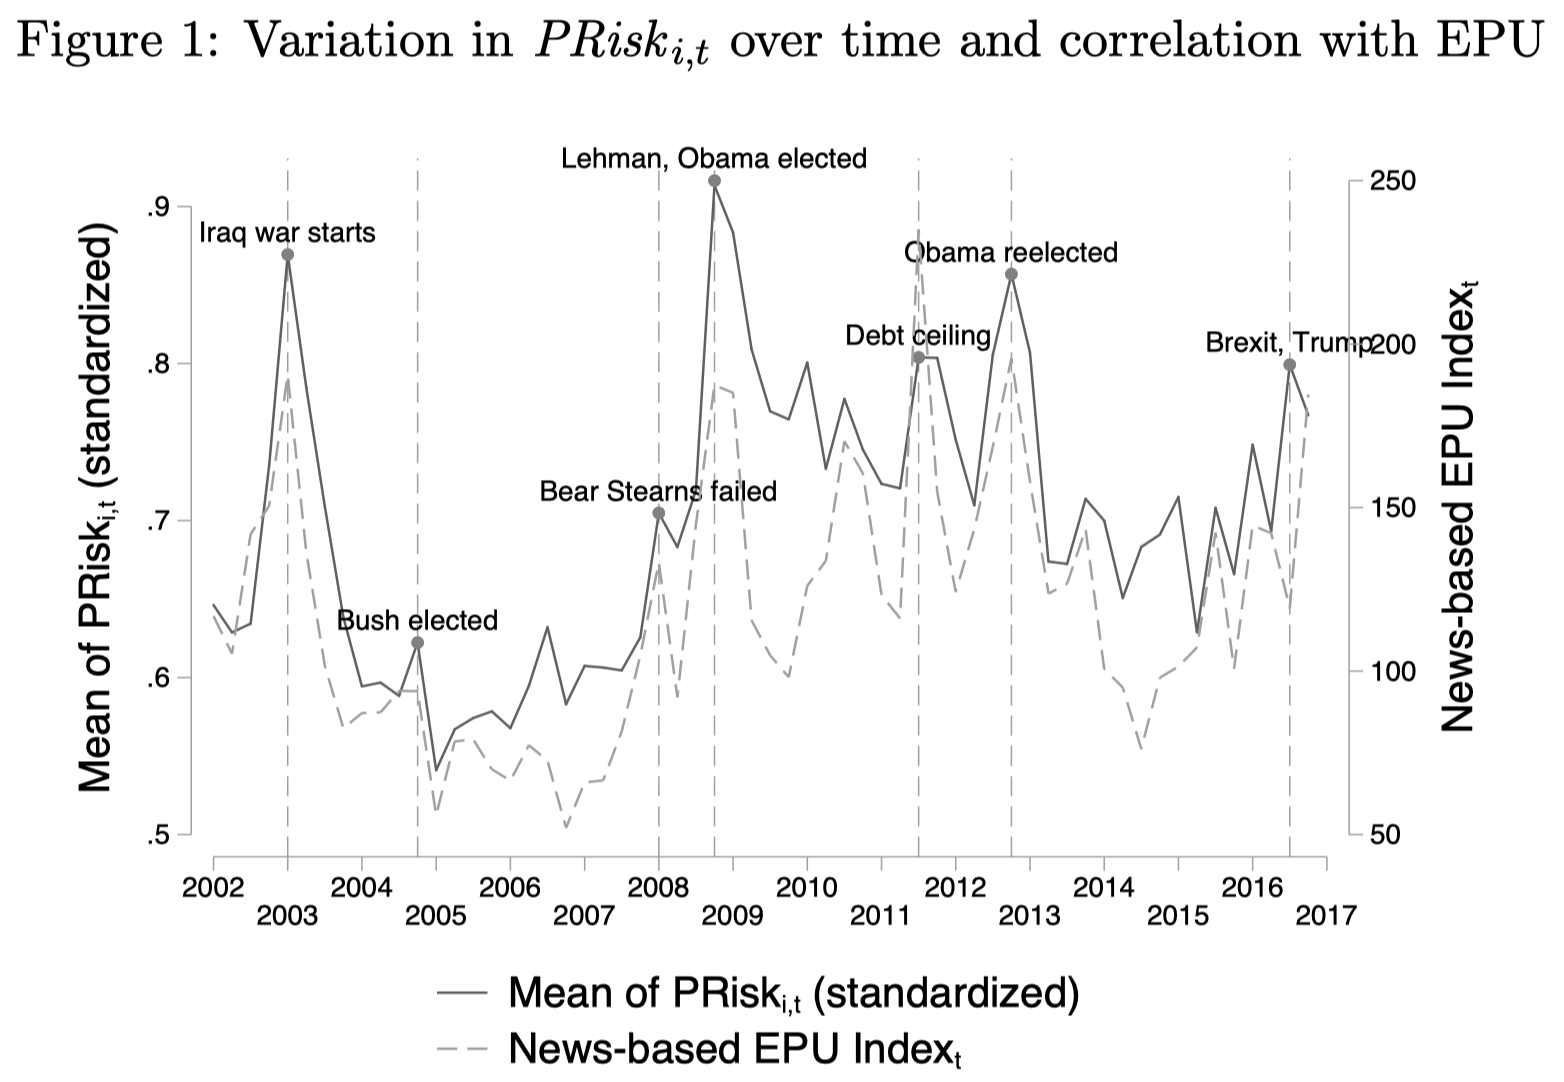
\includegraphics[scale=0.35]{Images/hassan_new1.png}
\end{center}
\end{frame}

\begin{frame}{Hassan et al. (QJE, 2019): using the dictionary}
\vspace{-7pt}
\begin{center}
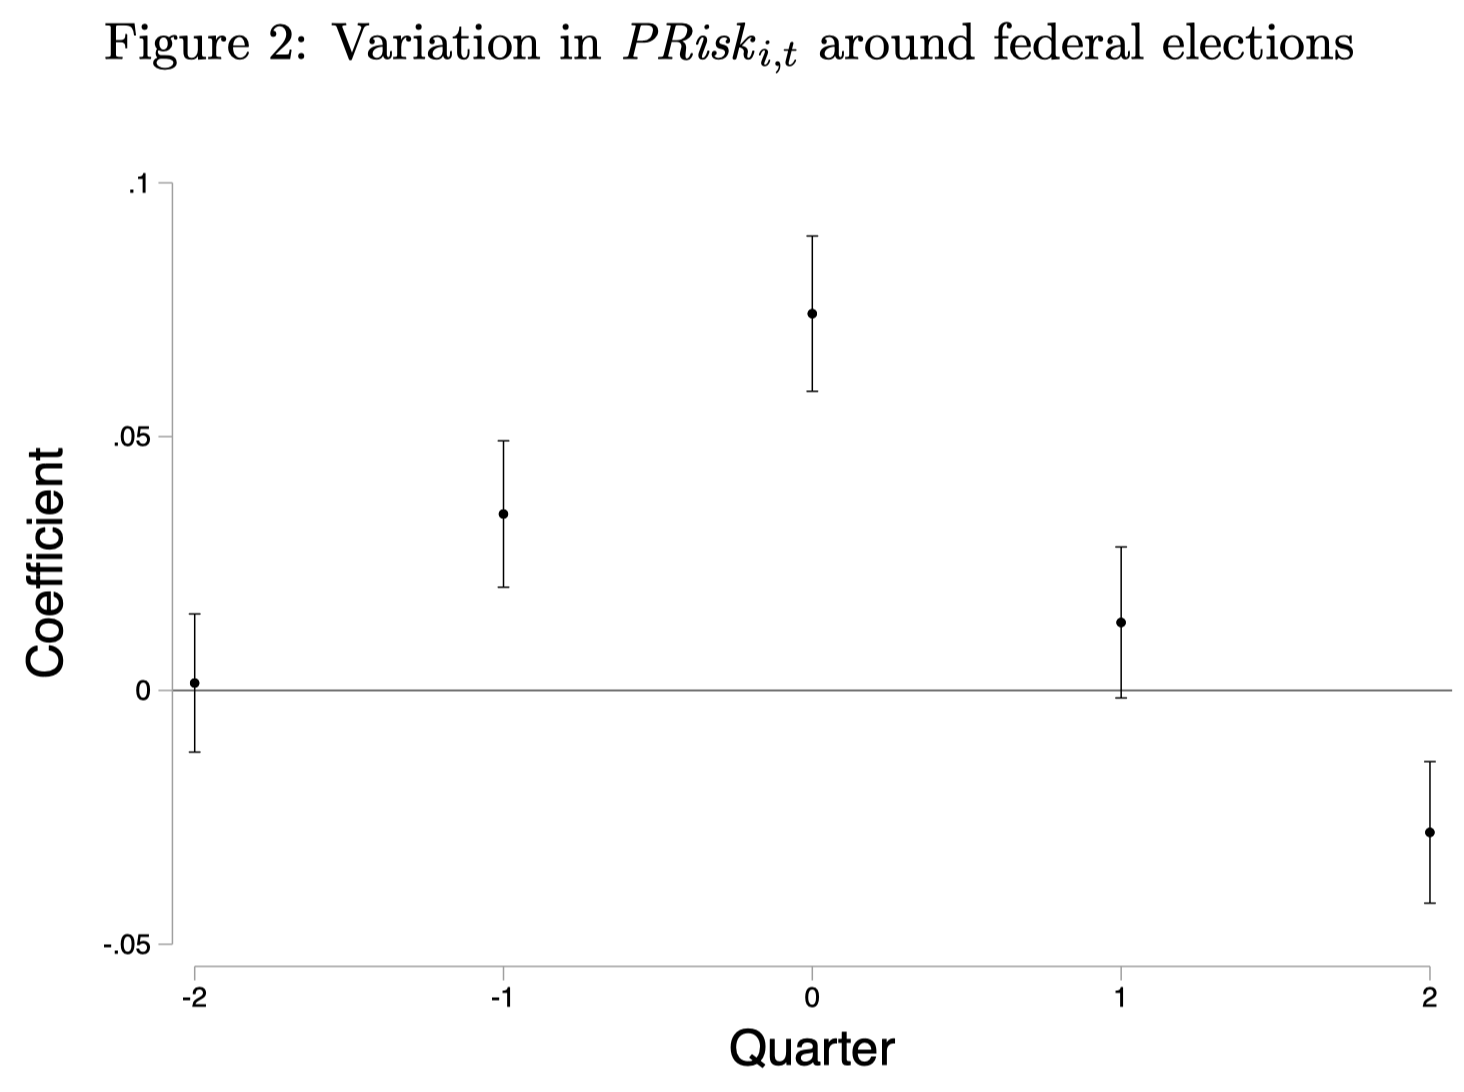
\includegraphics[scale=0.35]{Images/hassan_new2.png}
\end{center}
\end{frame}

\begin{frame}{Hassan et al. (QJE, 2019): using the dictionary}
\vspace{-7pt}
\begin{center}
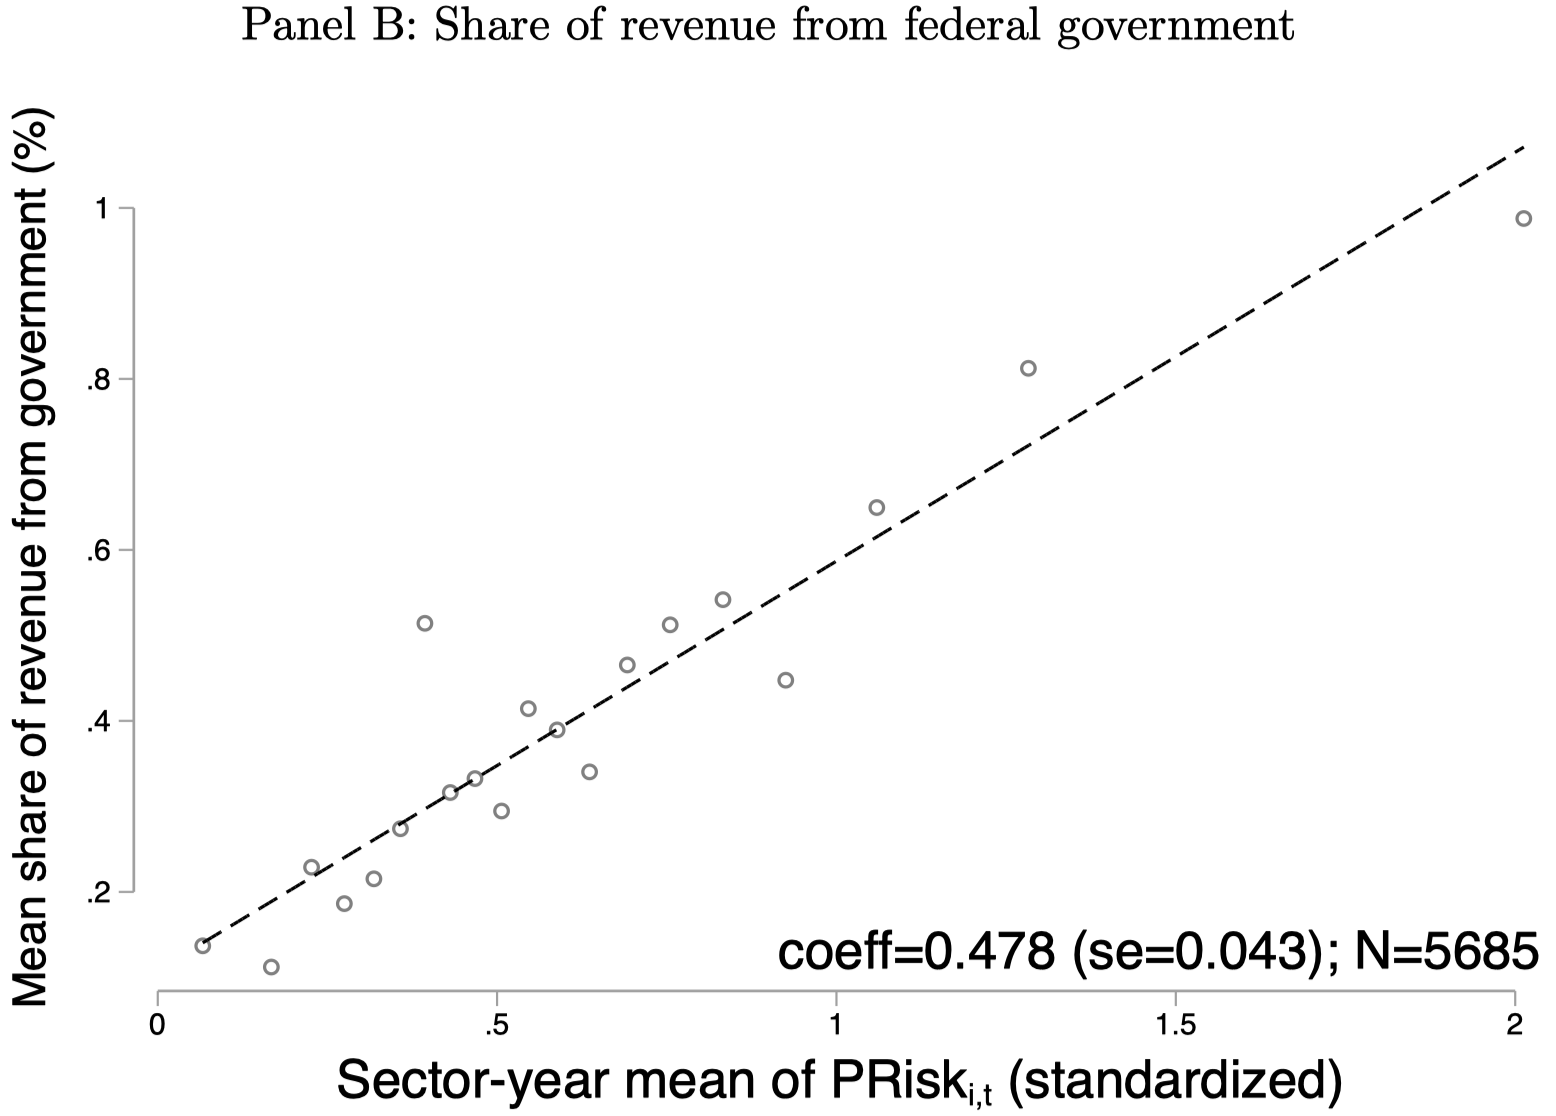
\includegraphics[scale=0.35]{Images/hassan_new3.png}
\end{center}
\end{frame}

\begin{frame}{Hassan et al. (QJE, 2019): using the dictionary}
\vspace{-7pt}
\begin{center}
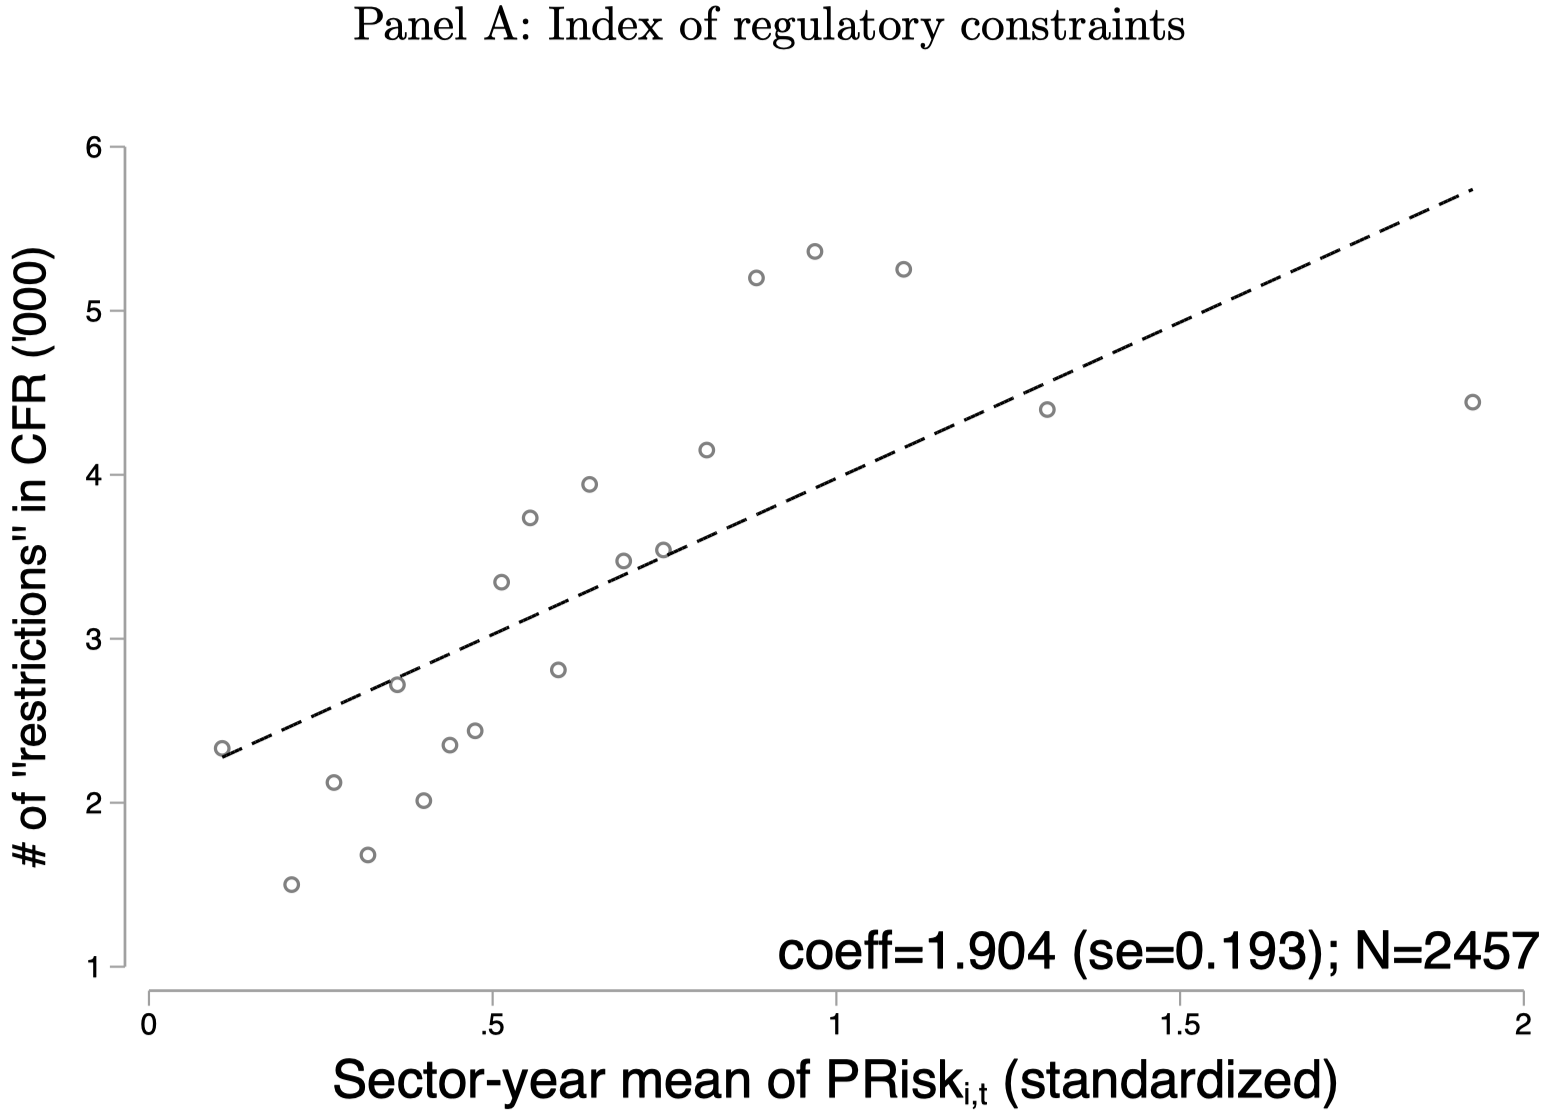
\includegraphics[scale=0.35]{Images/hassan_new4.png}
\end{center}
\end{frame}

\begin{frame}{More on dictionary-based methods: sentiment analysis}
\begin{itemize}
\setlength{\itemsep}{0.8em}
\item Sentiment analysis is a subfield of NLP that identifies and extracts opinions and sentiments from texts
\pause
\item Understanding emotions from text is challenging. Even humans can get misled, so do not expect a 100\% accuracy from computers
\item A text may contain multiple sentiments at once. E.g., \\
\vspace{2pt}
\textcolor{blue}{\textit{``The intent behind the final season of Game of Thrones\\
was great, but it could have been way better''}}
\item How do we conclude whether the review is positive or negative?
\item Also, computers cannot comprehend figurative speech, or understand the use of similes, metaphors, hyperboles, etc.
\pause
\item Two tools:
\vspace{4pt}
\begin{itemize}
\setlength{\itemsep}{0.3em}
\item Linguistic Inquiry and Word Count (LIWC)
\item Valence Aware Dictionary and sEntiment Reasoner (VADER)
\end{itemize}
\end{itemize}
\end{frame}


\begin{frame}{Linquistic Inquiry and Word Count (LIWC)}
\begin{itemize}
\setlength{\itemsep}{1em}
\item Created by Pennebaker et al. (see \textcolor{blue}{http://www.liwc.net)}
\item Uses a dictionary to calculate the percentage of words in the text that match each of up to 82 language dimensions
\item Consists of about 4,500 words and word stems, each defining one or more word categories or sub-dictionaries (non-exclusive)
\item E.g., the word ``cried'' is part of five word categories: sadness, negative emotion, overall affect, verb, and past tense verb.
\item Observing the token cried causes each of these five sub-dictionaries scale scores to be incremented
\item Hierarchy of categories: ``anger'' are part of an \textcolor{blue}{emotion} category and a \textcolor{blue}{negative emotion} subcategory
\end{itemize}
\end{frame}

\begin{frame}{Ex: emotional vs. cognitive processing in U.S. Congress}
\begin{center}
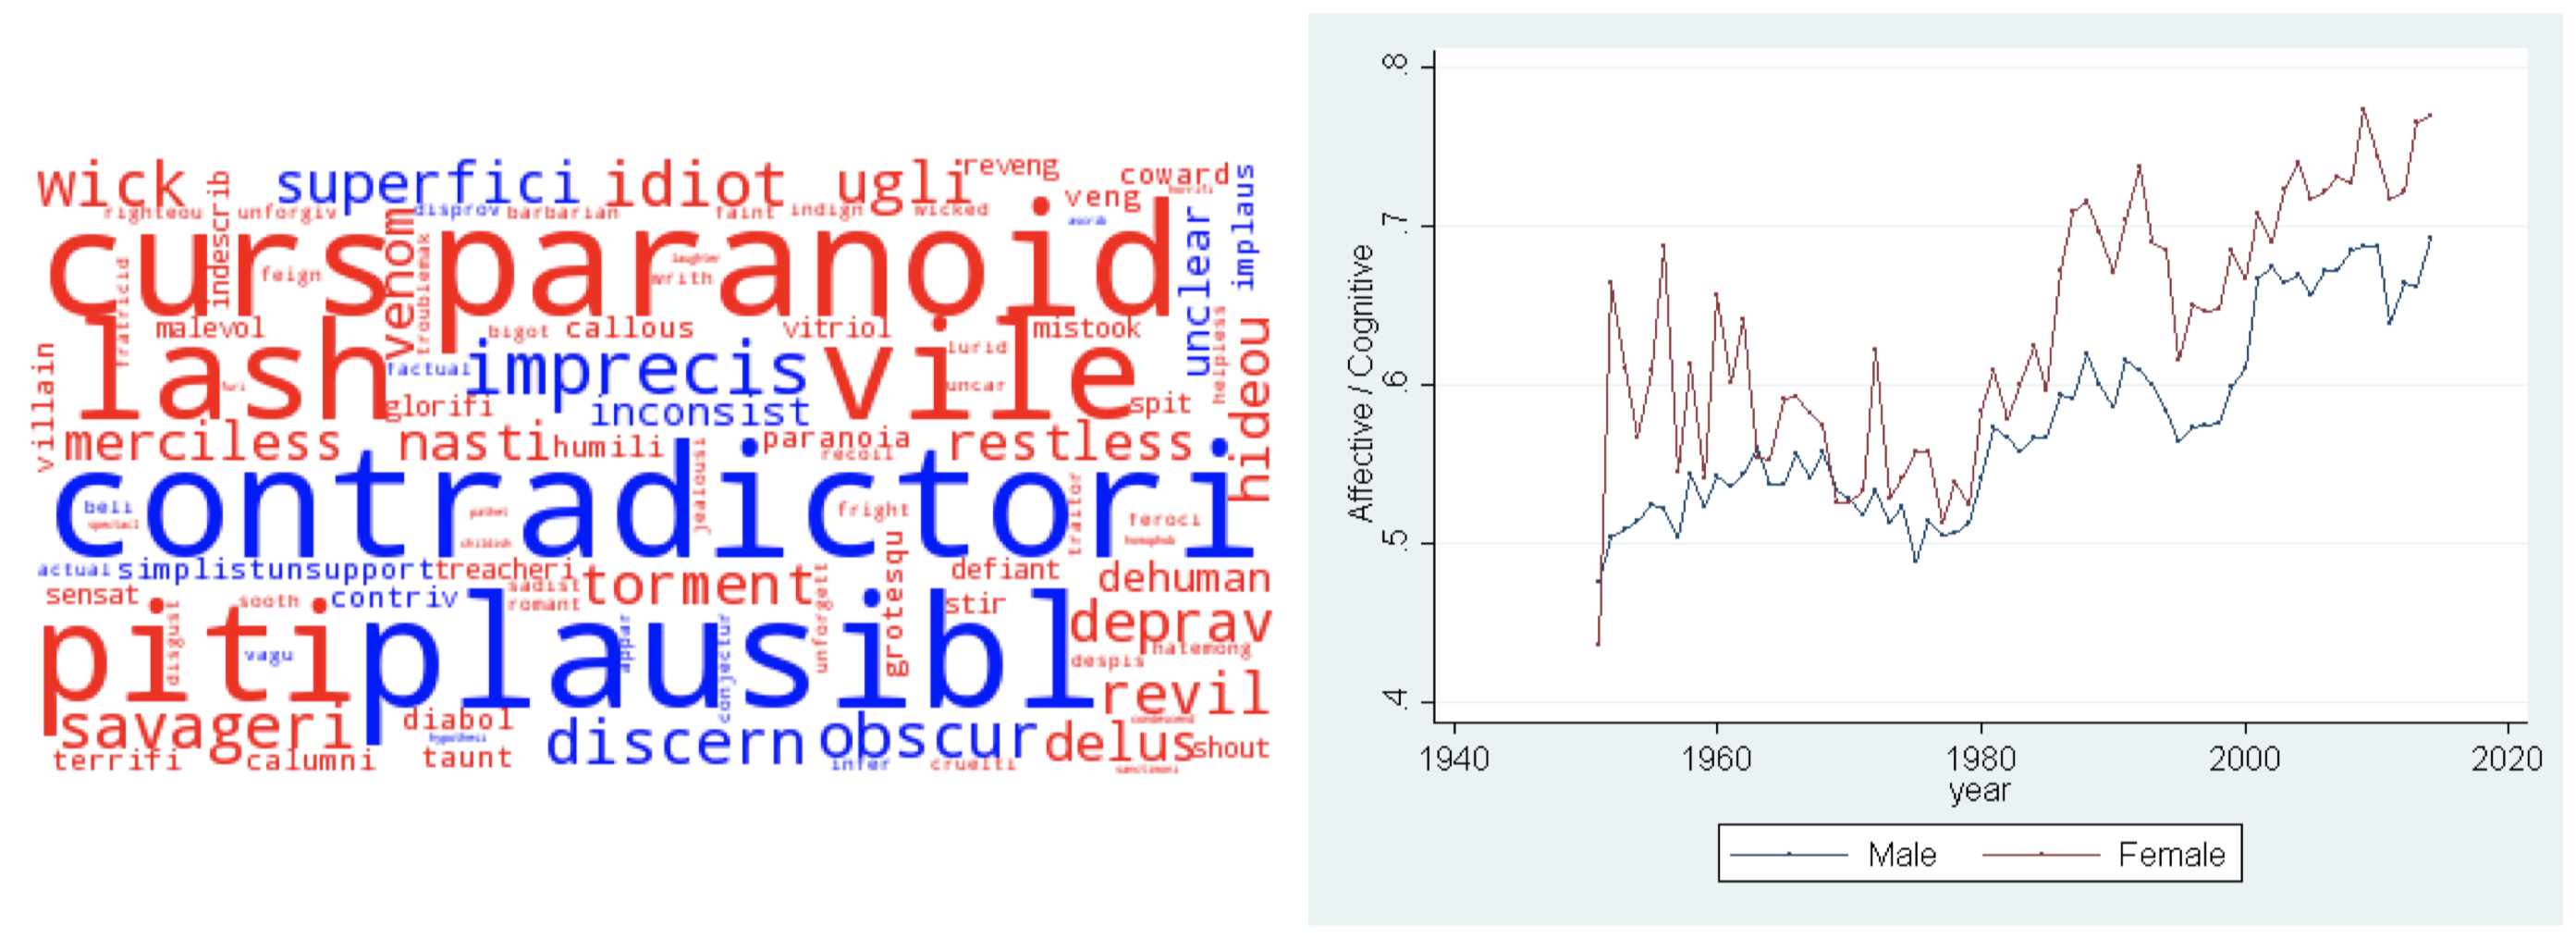
\includegraphics[scale=0.22]{Images/gennaro}
\vspace{10pt}
\normalsize{Source: Gennaro, Ash, and Loewen (2019)}
\end{center}

\end{frame}


\end{document}

